% !TEX root = z_output/_Goodwillie.tex

\documentclass[11pt]{article}
\usepackage{fullpage}
\usepackage{amsmath,amsthm,amssymb}
\usepackage{mathrsfs,nicefrac}
\usepackage{amssymb}
\usepackage{epsfig}
\usepackage[all,2cell]{xy}
\usepackage{sseq}
\usepackage{tocloft}
\usepackage{cancel}
\usepackage[strict]{changepage}
\usepackage{color}
\usepackage{tikz}
\usepackage{extpfeil}
\usepackage{version}
\usepackage{framed}
\definecolor{shadecolor}{rgb}{.925,0.925,0.925}

%\usepackage{ifthen}
%Used for disabling hyperref
\ifx\dontloadhyperref\undefined
%\usepackage[pdftex,pdfborder={0 0 0 [1 1]}]{hyperref}
\usepackage[pdftex,pdfborder={0 0 .5 [1 1]}]{hyperref}
\else
\providecommand{\texorpdfstring}[2]{#1}
\fi
%>>>>>>>>>>>>>>>>>>>>>>>>>>>>>>
%<<<        Versions        <<<
%>>>>>>>>>>>>>>>>>>>>>>>>>>>>>>
%Add in the following line to include all the versions.
%\def\excludeversion#1{\includeversion{#1}}

%>>>>>>>>>>>>>>>>>>>>>>>>>>>>>>
%<<<       Better ToC       <<<
%>>>>>>>>>>>>>>>>>>>>>>>>>>>>>>
\setlength{\cftbeforesecskip}{0.5ex}

%>>>>>>>>>>>>>>>>>>>>>>>>>>>>>>
%<<<      Hyperref mod      <<<
%>>>>>>>>>>>>>>>>>>>>>>>>>>>>>>

%needs more testing
\newcounter{dummyforrefstepcounter}
\newcommand{\labelRIGHTHERE}[1]
{\refstepcounter{dummyforrefstepcounter}\label{#1}}


%>>>>>>>>>>>>>>>>>>>>>>>>>>>>>>
%<<<  Theorem Environments  <<<
%>>>>>>>>>>>>>>>>>>>>>>>>>>>>>>
\ifx\dontloaddefinitionsoftheoremenvironments\undefined
\theoremstyle{plain}
\newtheorem{thm}{Theorem}[section]
\newtheorem*{thm*}{Theorem}
\newtheorem{lem}[thm]{Lemma}
\newtheorem*{lem*}{Lemma}
\newtheorem{prop}[thm]{Proposition}
\newtheorem*{prop*}{Proposition}
\newtheorem{cor}[thm]{Corollary}
\newtheorem*{cor*}{Corollary}
\newtheorem{defprop}[thm]{Definition-Proposition}
\newtheorem*{punchline}{Punchline}
\newtheorem*{conjecture}{Conjecture}
\newtheorem*{claim}{Claim}

\theoremstyle{definition}
\newtheorem{defn}{Definition}[section]
\newtheorem*{defn*}{Definition}
\newtheorem{exmp}{Example}[section]
\newtheorem*{exmp*}{Example}
\newtheorem*{exmps*}{Examples}
\newtheorem*{nonexmp*}{Non-example}
\newtheorem{asspt}{Assumption}[section]
\newtheorem{notation}{Notation}[section]
\newtheorem{exercise}{Exercise}[section]
\newtheorem*{fact*}{Fact}
\newtheorem*{rmk*}{Remark}
\newtheorem{fact}{Fact}
\newtheorem*{aside}{Aside}
\newtheorem*{question}{Question}
\newtheorem*{answer}{Answer}

\else\relax\fi

%>>>>>>>>>>>>>>>>>>>>>>>>>>>>>>
%<<<      Fields, etc.      <<<
%>>>>>>>>>>>>>>>>>>>>>>>>>>>>>>
\DeclareSymbolFont{AMSb}{U}{msb}{m}{n}
\DeclareMathSymbol{\N}{\mathbin}{AMSb}{"4E}
\DeclareMathSymbol{\Octonions}{\mathbin}{AMSb}{"4F}
\DeclareMathSymbol{\Z}{\mathbin}{AMSb}{"5A}
\DeclareMathSymbol{\R}{\mathbin}{AMSb}{"52}
\DeclareMathSymbol{\Q}{\mathbin}{AMSb}{"51}
\DeclareMathSymbol{\PP}{\mathbin}{AMSb}{"50}
\DeclareMathSymbol{\I}{\mathbin}{AMSb}{"49}
\DeclareMathSymbol{\C}{\mathbin}{AMSb}{"43}
\DeclareMathSymbol{\A}{\mathbin}{AMSb}{"41}
\DeclareMathSymbol{\F}{\mathbin}{AMSb}{"46}
\DeclareMathSymbol{\G}{\mathbin}{AMSb}{"47}
\DeclareMathSymbol{\Quaternions}{\mathbin}{AMSb}{"48}


%>>>>>>>>>>>>>>>>>>>>>>>>>>>>>>
%<<<       Operators        <<<
%>>>>>>>>>>>>>>>>>>>>>>>>>>>>>>
\DeclareMathOperator{\ad}{\textbf{ad}}
\DeclareMathOperator{\coker}{coker}
\renewcommand{\ker}{\textup{ker}\,}
\DeclareMathOperator{\End}{End}
\DeclareMathOperator{\Aut}{Aut}
\DeclareMathOperator{\Hom}{Hom}
\DeclareMathOperator{\Maps}{Maps}
\DeclareMathOperator{\Mor}{Mor}
\DeclareMathOperator{\Gal}{Gal}
\DeclareMathOperator{\Ext}{Ext}
\DeclareMathOperator{\Tor}{Tor}
\DeclareMathOperator{\Map}{Map}
\DeclareMathOperator{\Der}{Der}
\DeclareMathOperator{\Rad}{Rad}
\DeclareMathOperator{\rank}{rank}
\DeclareMathOperator{\ArfInvariant}{Arf}
\DeclareMathOperator{\KervaireInvariant}{Ker}
\DeclareMathOperator{\im}{im}
\DeclareMathOperator{\coim}{coim}
\DeclareMathOperator{\trace}{tr}
\DeclareMathOperator{\supp}{supp}
\DeclareMathOperator{\ann}{ann}
\DeclareMathOperator{\spec}{Spec}
\DeclareMathOperator{\SPEC}{\textbf{Spec}}
\DeclareMathOperator{\proj}{Proj}
\DeclareMathOperator{\PROJ}{\textbf{Proj}}
\DeclareMathOperator{\fiber}{F}
\DeclareMathOperator{\cofiber}{C}
\DeclareMathOperator{\cone}{cone}
\DeclareMathOperator{\skel}{sk}
\DeclareMathOperator{\coskel}{cosk}
\DeclareMathOperator{\conn}{conn}
\DeclareMathOperator{\colim}{colim}
\DeclareMathOperator{\limit}{lim}
\DeclareMathOperator{\ch}{ch}
\DeclareMathOperator{\Vect}{Vect}
\DeclareMathOperator{\GrthGrp}{GrthGp}
\DeclareMathOperator{\Sym}{Sym}
\DeclareMathOperator{\Prob}{\mathbb{P}}
\DeclareMathOperator{\Exp}{\mathbb{E}}
\DeclareMathOperator{\GeomMean}{\mathbb{G}}
\DeclareMathOperator{\Var}{Var}
\DeclareMathOperator{\Cov}{Cov}
\DeclareMathOperator{\Sp}{Sp}
\DeclareMathOperator{\Seq}{Seq}
\DeclareMathOperator{\Cyl}{Cyl}
\DeclareMathOperator{\Ev}{Ev}
\DeclareMathOperator{\sh}{sh}
\DeclareMathOperator{\intHom}{\underline{Hom}}
\DeclareMathOperator{\Frac}{frac}



%>>>>>>>>>>>>>>>>>>>>>>>>>>>>>>
%<<<   Cohomology Theories  <<<
%>>>>>>>>>>>>>>>>>>>>>>>>>>>>>>
\DeclareMathOperator{\KR}{{K\R}}
\DeclareMathOperator{\KO}{{KO}}
\DeclareMathOperator{\K}{{K}}
\DeclareMathOperator{\OmegaO}{{\Omega_{\Octonions}}}

%>>>>>>>>>>>>>>>>>>>>>>>>>>>>>>
%<<<   Algebraic Geometry   <<<
%>>>>>>>>>>>>>>>>>>>>>>>>>>>>>>
\DeclareMathOperator{\Spec}{Spec}
\DeclareMathOperator{\Proj}{Proj}
\DeclareMathOperator{\Sing}{Sing}
\DeclareMathOperator{\shfHom}{\mathscr{H}\textit{\!\!om}}
\DeclareMathOperator{\WeilDivisors}{{Div}}
\DeclareMathOperator{\CartierDivisors}{{CaDiv}}
\DeclareMathOperator{\PrincipalWeilDivisors}{{PrDiv}}
\DeclareMathOperator{\LocallyPrincipalWeilDivisors}{{LPDiv}}
\DeclareMathOperator{\PrincipalCartierDivisors}{{PrCaDiv}}
\DeclareMathOperator{\DivisorClass}{{Cl}}
\DeclareMathOperator{\CartierClass}{{CaCl}}
\DeclareMathOperator{\Picard}{{Pic}}
\DeclareMathOperator{\Frob}{Frob}


%>>>>>>>>>>>>>>>>>>>>>>>>>>>>>>
%<<<  Mathematical Objects  <<<
%>>>>>>>>>>>>>>>>>>>>>>>>>>>>>>
\newcommand{\sll}{\mathfrak{sl}}
\newcommand{\gl}{\mathfrak{gl}}
\newcommand{\GL}{\mbox{GL}}
\newcommand{\PGL}{\mbox{PGL}}
\newcommand{\SL}{\mbox{SL}}
\newcommand{\Mat}{\mbox{Mat}}
\newcommand{\Gr}{\textup{Gr}}
\newcommand{\Squ}{\textup{Sq}}
\newcommand{\catSet}{\textit{Sets}}
\newcommand{\RP}{{\R\PP}}
\newcommand{\CP}{{\C\PP}}
\newcommand{\Steen}{\mathscr{A}}
\newcommand{\Orth}{\textup{\textbf{O}}}

%>>>>>>>>>>>>>>>>>>>>>>>>>>>>>>
%<<<  Mathematical Symbols  <<<
%>>>>>>>>>>>>>>>>>>>>>>>>>>>>>>
\newcommand{\DASH}{\textup{---}}
\newcommand{\op}{\textup{op}}
\newcommand{\CW}{\textup{CW}}
\newcommand{\ob}{\textup{ob}\,}
\newcommand{\ho}{\textup{ho}}
\newcommand{\st}{\textup{st}}
\newcommand{\id}{\textup{id}}
\newcommand{\Bullet}{\ensuremath{\bullet} }
\newcommand{\sprod}{\wedge}

%>>>>>>>>>>>>>>>>>>>>>>>>>>>>>>
%<<<      Some Arrows       <<<
%>>>>>>>>>>>>>>>>>>>>>>>>>>>>>>
\newcommand{\nt}{\Longrightarrow}
\let\shortmapsto\mapsto
\let\mapsto\longmapsto
\newcommand{\mapsfrom}{\,\reflectbox{$\mapsto$}\ }
\newcommand{\bigrightsquig}{\scalebox{2}{\ensuremath{\rightsquigarrow}}}
\newcommand{\bigleftsquig}{\reflectbox{\scalebox{2}{\ensuremath{\rightsquigarrow}}}}

%\newcommand{\cofibration}{\xhookrightarrow{\phantom{\ \,{\sim\!}\ \ }}}
%\newcommand{\fibration}{\xtwoheadrightarrow{\phantom{\sim\!}}}
%\newcommand{\acycliccofibration}{\xhookrightarrow{\ \,{\sim\!}\ \ }}
%\newcommand{\acyclicfibration}{\xtwoheadrightarrow{\sim\!}}
%\newcommand{\leftcofibration}{\xhookleftarrow{\phantom{\ \,{\sim\!}\ \ }}}
%\newcommand{\leftfibration}{\xtwoheadleftarrow{\phantom{\sim\!}}}
%\newcommand{\leftacycliccofibration}{\xhookleftarrow{\ \ {\sim\!}\,\ }}
%\newcommand{\leftacyclicfibration}{\xtwoheadleftarrow{\sim\!}}
%\newcommand{\weakequiv}{\xrightarrow{\ \,\sim\,\ }}
%\newcommand{\leftweakequiv}{\xleftarrow{\ \,\sim\,\ }}

\newcommand{\cofibration}
{\xhookrightarrow{\phantom{\ \,{\raisebox{-.3ex}[0ex][0ex]{\scriptsize$\sim$}\!}\ \ }}}
\newcommand{\fibration}
{\xtwoheadrightarrow{\phantom{\raisebox{-.3ex}[0ex][0ex]{\scriptsize$\sim$}\!}}}
\newcommand{\acycliccofibration}
{\xhookrightarrow{\ \,{\raisebox{-.55ex}[0ex][0ex]{\scriptsize$\sim$}\!}\ \ }}
\newcommand{\acyclicfibration}
{\xtwoheadrightarrow{\raisebox{-.6ex}[0ex][0ex]{\scriptsize$\sim$}\!}}
\newcommand{\leftcofibration}
{\xhookleftarrow{\phantom{\ \,{\raisebox{-.3ex}[0ex][0ex]{\scriptsize$\sim$}\!}\ \ }}}
\newcommand{\leftfibration}
{\xtwoheadleftarrow{\phantom{\raisebox{-.3ex}[0ex][0ex]{\scriptsize$\sim$}\!}}}
\newcommand{\leftacycliccofibration}
{\xhookleftarrow{\ \ {\raisebox{-.55ex}[0ex][0ex]{\scriptsize$\sim$}\!}\,\ }}
\newcommand{\leftacyclicfibration}
{\xtwoheadleftarrow{\raisebox{-.6ex}[0ex][0ex]{\scriptsize$\sim$}\!}}
\newcommand{\weakequiv}
{\xrightarrow{\ \,\raisebox{-.3ex}[0ex][0ex]{\scriptsize$\sim$}\,\ }}
\newcommand{\leftweakequiv}
{\xleftarrow{\ \,\raisebox{-.3ex}[0ex][0ex]{\scriptsize$\sim$}\,\ }}

%>>>>>>>>>>>>>>>>>>>>>>>>>>>>>>
%<<<    xymatrix Arrows     <<<
%>>>>>>>>>>>>>>>>>>>>>>>>>>>>>>
\newdir{ >}{{}*!/-5pt/@{>}}
\newcommand{\xycof}{\ar@{ >->}}
\newcommand{\xycofib}{\ar@{^{(}->}}
\newcommand{\xycofibdown}{\ar@{_{(}->}}
\newcommand{\xyfib}{\ar@{->>}}
\newcommand{\xymapsto}{\ar@{|->}}

%>>>>>>>>>>>>>>>>>>>>>>>>>>>>>>
%<<<     Greek Letters      <<<
%>>>>>>>>>>>>>>>>>>>>>>>>>>>>>>
%\newcommand{\oldphi}{\phi}
%\renewcommand{\phi}{\varphi}
\let\oldphi\phi
\let\phi\varphi
\renewcommand{\to}{\longrightarrow}
\newcommand{\from}{\longleftarrow}
\newcommand{\eps}{\varepsilon}

%>>>>>>>>>>>>>>>>>>>>>>>>>>>>>>
%<<<  1st-4th & parentheses <<<
%>>>>>>>>>>>>>>>>>>>>>>>>>>>>>>
\newcommand{\first}{^\text{st}}
\newcommand{\second}{^\text{nd}}
\newcommand{\third}{^\text{rd}}
\newcommand{\fourth}{^\text{th}}
\newcommand{\ZEROTH}{$0^\text{th}$ }
\newcommand{\FIRST}{$1^\text{st}$ }
\newcommand{\SECOND}{$2^\text{nd}$ }
\newcommand{\THIRD}{$3^\text{rd}$ }
\newcommand{\FOURTH}{$4^\text{th}$ }
\newcommand{\iTH}{$i^\text{th}$ }
\newcommand{\jTH}{$j^\text{th}$ }
\newcommand{\nTH}{$n^\text{th}$ }

%>>>>>>>>>>>>>>>>>>>>>>>>>>>>>>
%<<<    upright commands    <<<
%>>>>>>>>>>>>>>>>>>>>>>>>>>>>>>
\newcommand{\upcol}{\textup{:}}
\newcommand{\upsemi}{\textup{;}}
\providecommand{\lparen}{\textup{(}}
\providecommand{\rparen}{\textup{)}}
\renewcommand{\lparen}{\textup{(}}
\renewcommand{\rparen}{\textup{)}}
\newcommand{\Iff}{\emph{iff} }

%>>>>>>>>>>>>>>>>>>>>>>>>>>>>>>
%<<<     Environments       <<<
%>>>>>>>>>>>>>>>>>>>>>>>>>>>>>>
\newcommand{\squishlist}
{ %\setlength{\topsep}{100pt} doesn't seem to do anything.
  \setlength{\itemsep}{.5pt}
  \setlength{\parskip}{0pt}
  \setlength{\parsep}{0pt}}
\newenvironment{itemise}{
\begin{list}{\textup{$\rightsquigarrow$}}
   {  \setlength{\topsep}{1mm}
      \setlength{\itemsep}{1pt}
      \setlength{\parskip}{0pt}
      \setlength{\parsep}{0pt}
   }
}{\end{list}\vspace{-.1cm}}
\newcommand{\INDENT}{\textbf{}\phantom{space}}
\renewcommand{\INDENT}{\rule{.7cm}{0cm}}

\newcommand{\itm}[1][$\rightsquigarrow$]{\item[{\makebox[.5cm][c]{\textup{#1}}}]}


%\newcommand{\rednote}[1]{{\color{red}#1}\makebox[0cm][l]{\scalebox{.1}{rednote}}}
%\newcommand{\bluenote}[1]{{\color{blue}#1}\makebox[0cm][l]{\scalebox{.1}{rednote}}}

\newcommand{\rednote}[1]
{{\color{red}#1}\makebox[0cm][l]{\scalebox{.1}{\rotatebox{90}{?????}}}}
\newcommand{\bluenote}[1]
{{\color{blue}#1}\makebox[0cm][l]{\scalebox{.1}{\rotatebox{90}{?????}}}}


\newcommand{\funcdef}[4]{\begin{align*}
#1&\to #2\\
#3&\mapsto#4
\end{align*}}

%\newcommand{\comment}[1]{}

%>>>>>>>>>>>>>>>>>>>>>>>>>>>>>>
%<<<       Categories       <<<
%>>>>>>>>>>>>>>>>>>>>>>>>>>>>>>
\newcommand{\Ens}{{\mathscr{E}ns}}
\DeclareMathOperator{\Sheaves}{{\mathsf{Shf}}}
\DeclareMathOperator{\Presheaves}{{\mathsf{PreShf}}}
\DeclareMathOperator{\Psh}{{\mathsf{Psh}}}
\DeclareMathOperator{\Shf}{{\mathsf{Shf}}}
\DeclareMathOperator{\Varieties}{{\mathsf{Var}}}
\DeclareMathOperator{\Schemes}{{\mathsf{Sch}}}
\DeclareMathOperator{\Rings}{{\mathsf{Rings}}}
\DeclareMathOperator{\AbGp}{{\mathsf{AbGp}}}
\DeclareMathOperator{\Modules}{{\mathsf{\!-Mod}}}
\DeclareMathOperator{\fgModules}{{\mathsf{\!-Mod}^{\textup{fg}}}}
\DeclareMathOperator{\QuasiCoherent}{{\mathsf{QCoh}}}
\DeclareMathOperator{\Coherent}{{\mathsf{Coh}}}
\DeclareMathOperator{\GSW}{{\mathcal{SW}^G}}
\DeclareMathOperator{\Burnside}{{\mathsf{Burn}}}
\DeclareMathOperator{\GSet}{{G\mathsf{Set}}}
\DeclareMathOperator{\FinGSet}{{G\mathsf{Set}^\textup{fin}}}
\DeclareMathOperator{\HSet}{{H\mathsf{Set}}}
\DeclareMathOperator{\Cat}{{\mathsf{Cat}}}
\DeclareMathOperator{\Fun}{{\mathsf{Fun}}}
\DeclareMathOperator{\Orb}{{\mathsf{Orb}}}
\DeclareMathOperator{\Set}{{\mathsf{Set}}}
\DeclareMathOperator{\sSet}{{\mathsf{sSet}}}
\DeclareMathOperator{\Top}{{\mathsf{Top}}}
\DeclareMathOperator{\GSpectra}{{G-\mathsf{Spectra}}}
\DeclareMathOperator{\Lan}{Lan}
\DeclareMathOperator{\Ran}{Ran}

%>>>>>>>>>>>>>>>>>>>>>>>>>>>>>>
%<<<     Script Letters     <<<
%>>>>>>>>>>>>>>>>>>>>>>>>>>>>>>
\newcommand{\scrQ}{\mathscr{Q}}
\newcommand{\scrW}{\mathscr{W}}
\newcommand{\scrE}{\mathscr{E}}
\newcommand{\scrR}{\mathscr{R}}
\newcommand{\scrT}{\mathscr{T}}
\newcommand{\scrY}{\mathscr{Y}}
\newcommand{\scrU}{\mathscr{U}}
\newcommand{\scrI}{\mathscr{I}}
\newcommand{\scrO}{\mathscr{O}}
\newcommand{\scrP}{\mathscr{P}}
\newcommand{\scrA}{\mathscr{A}}
\newcommand{\scrS}{\mathscr{S}}
\newcommand{\scrD}{\mathscr{D}}
\newcommand{\scrF}{\mathscr{F}}
\newcommand{\scrG}{\mathscr{G}}
\newcommand{\scrH}{\mathscr{H}}
\newcommand{\scrJ}{\mathscr{J}}
\newcommand{\scrK}{\mathscr{K}}
\newcommand{\scrL}{\mathscr{L}}
\newcommand{\scrZ}{\mathscr{Z}}
\newcommand{\scrX}{\mathscr{X}}
\newcommand{\scrC}{\mathscr{C}}
\newcommand{\scrV}{\mathscr{V}}
\newcommand{\scrB}{\mathscr{B}}
\newcommand{\scrN}{\mathscr{N}}
\newcommand{\scrM}{\mathscr{M}}

%>>>>>>>>>>>>>>>>>>>>>>>>>>>>>>
%<<<     Fractur Letters    <<<
%>>>>>>>>>>>>>>>>>>>>>>>>>>>>>>
\newcommand{\frakQ}{\mathfrak{Q}}
\newcommand{\frakW}{\mathfrak{W}}
\newcommand{\frakE}{\mathfrak{E}}
\newcommand{\frakR}{\mathfrak{R}}
\newcommand{\frakT}{\mathfrak{T}}
\newcommand{\frakY}{\mathfrak{Y}}
\newcommand{\frakU}{\mathfrak{U}}
\newcommand{\frakI}{\mathfrak{I}}
\newcommand{\frakO}{\mathfrak{O}}
\newcommand{\frakP}{\mathfrak{P}}
\newcommand{\frakA}{\mathfrak{A}}
\newcommand{\frakS}{\mathfrak{S}}
\newcommand{\frakD}{\mathfrak{D}}
\newcommand{\frakF}{\mathfrak{F}}
\newcommand{\frakG}{\mathfrak{G}}
\newcommand{\frakH}{\mathfrak{H}}
\newcommand{\frakJ}{\mathfrak{J}}
\newcommand{\frakK}{\mathfrak{K}}
\newcommand{\frakL}{\mathfrak{L}}
\newcommand{\frakZ}{\mathfrak{Z}}
\newcommand{\frakX}{\mathfrak{X}}
\newcommand{\frakC}{\mathfrak{C}}
\newcommand{\frakV}{\mathfrak{V}}
\newcommand{\frakB}{\mathfrak{B}}
\newcommand{\frakN}{\mathfrak{N}}
\newcommand{\frakM}{\mathfrak{M}}

\newcommand{\frakq}{\mathfrak{q}}
\newcommand{\frakw}{\mathfrak{w}}
\newcommand{\frake}{\mathfrak{e}}
\newcommand{\frakr}{\mathfrak{r}}
\newcommand{\frakt}{\mathfrak{t}}
\newcommand{\fraky}{\mathfrak{y}}
\newcommand{\fraku}{\mathfrak{u}}
\newcommand{\fraki}{\mathfrak{i}}
\newcommand{\frako}{\mathfrak{o}}
\newcommand{\frakp}{\mathfrak{p}}
\newcommand{\fraka}{\mathfrak{a}}
\newcommand{\fraks}{\mathfrak{s}}
\newcommand{\frakd}{\mathfrak{d}}
\newcommand{\frakf}{\mathfrak{f}}
\newcommand{\frakg}{\mathfrak{g}}
\newcommand{\frakh}{\mathfrak{h}}
\newcommand{\frakj}{\mathfrak{j}}
\newcommand{\frakk}{\mathfrak{k}}
\newcommand{\frakl}{\mathfrak{l}}
\newcommand{\frakz}{\mathfrak{z}}
\newcommand{\frakx}{\mathfrak{x}}
\newcommand{\frakc}{\mathfrak{c}}
\newcommand{\frakv}{\mathfrak{v}}
\newcommand{\frakb}{\mathfrak{b}}
\newcommand{\frakn}{\mathfrak{n}}
\newcommand{\frakm}{\mathfrak{m}}

%>>>>>>>>>>>>>>>>>>>>>>>>>>>>>>
%<<<  Caligraphic Letters   <<<
%>>>>>>>>>>>>>>>>>>>>>>>>>>>>>>
\newcommand{\calQ}{\mathcal{Q}}
\newcommand{\calW}{\mathcal{W}}
\newcommand{\calE}{\mathcal{E}}
\newcommand{\calR}{\mathcal{R}}
\newcommand{\calT}{\mathcal{T}}
\newcommand{\calY}{\mathcal{Y}}
\newcommand{\calU}{\mathcal{U}}
\newcommand{\calI}{\mathcal{I}}
\newcommand{\calO}{\mathcal{O}}
\newcommand{\calP}{\mathcal{P}}
\newcommand{\calA}{\mathcal{A}}
\newcommand{\calS}{\mathcal{S}}
\newcommand{\calD}{\mathcal{D}}
\newcommand{\calF}{\mathcal{F}}
\newcommand{\calG}{\mathcal{G}}
\newcommand{\calH}{\mathcal{H}}
\newcommand{\calJ}{\mathcal{J}}
\newcommand{\calK}{\mathcal{K}}
\newcommand{\calL}{\mathcal{L}}
\newcommand{\calZ}{\mathcal{Z}}
\newcommand{\calX}{\mathcal{X}}
\newcommand{\calC}{\mathcal{C}}
\newcommand{\calV}{\mathcal{V}}
\newcommand{\calB}{\mathcal{B}}
\newcommand{\calN}{\mathcal{N}}
\newcommand{\calM}{\mathcal{M}}

%>>>>>>>>>>>>>>>>>>>>>>>>>>>>>>
%<<<<<<<<<DEPRECIATED<<<<<<<<<<
%>>>>>>>>>>>>>>>>>>>>>>>>>>>>>>

%%% From Kac's template
% 1-inch margins, from fullpage.sty by H.Partl, Version 2, Dec. 15, 1988.
%\topmargin 0pt
%\advance \topmargin by -\headheight
%\advance \topmargin by -\headsep
%\textheight 9.1in
%\oddsidemargin 0pt
%\evensidemargin \oddsidemargin
%\marginparwidth 0.5in
%\textwidth 6.5in
%
%\parindent 0in
%\parskip 1.5ex
%%\renewcommand{\baselinestretch}{1.25}

%%% From the net
%\newcommand{\pullbackcorner}[1][dr]{\save*!/#1+1.2pc/#1:(1,-1)@^{|-}\restore}
%\newcommand{\pushoutcorner}[1][dr]{\save*!/#1-1.2pc/#1:(-1,1)@^{|-}\restore}









\usetikzlibrary{arrows,positioning}
\usetikzlibrary{decorations.markings}
\usetikzlibrary{calc}
\tikzset{
 >=stealth',
 shorten <=-5pt,
 shorten >=-5pt,
 shape=circle
}

%\newcommand{\overedge}[3]{\path[#1] \path[->] (#2) edge [-,line width=3pt,draw=white] (#3) edge (#3);}

%\def\excludeversion#1{\includeversion{#1}}
\excludeversion{Calculus I}
\excludeversion{Calculus II}
\excludeversion{Calculus III}

\excludeversion{Note on derivatives}

\newcommand{\TF}{\raisebox{.091em}{$\therefore$}\,}
\newcommand\ST{\rule[-.25em]{0pt}{1.25em}}
\DeclareMathOperator{\dist}{dist}
\DeclareMathOperator{\cartesianness}{cart}
\UseAllTwocells
\begin{document}
\begin{Calculus I}
\section*{Calculus I}
\begin{itemise}
\setlength{\parindent}{.25in}
\item A homotopical functor $\scru\to\scrt$ is:
\begin{itemize}\squishlist
\setlength{\parindent}{.25in}
\item  \textbf{excisive} if it sends (homotopy) pushouts to (homotopy) pullbacks.
\item \textbf{reduced} if it sends the final object to a contractible space. (?)
\end{itemize}
\item We can  form the reduction $\widetilde{F}$ of a functor $F$ by defining $\widetilde{F}:Y\mapsto\fiber(F(Y)\to F(*))$.
\item If the (homotopical) functor is excisive and reduced, we call it \textbf{linear}, and the spaces $F(S^i)$ form an $\Omega$-spectrum, called the coefficient spectrum.
\item If $F$ is only reduced, the $F(S^i)$ form a prespectrum, whose associated spectrum is $\partial F(*)$, the derivative of $F$ at $*$.
\item The differential of $F$ at $*$ is the (possibly nonlinear) functor
\[D_*F:Y\mapsto\hocolim\left(\widetilde{F}(Y)\to\Omega\widetilde{F}(SY)\to\Omega^2\widetilde{F}(S^2Y)\to\cdots \right)\]
When $F$ is \emph{stably excisive}, $D_*F$ is linear with coefficient spectrum $\partial F(*)$, and is the best linear approximation to $\widetilde{F}$: there's a natural transformation $\widetilde{F}\nt D_*F$, and its fiber, a functor $\scru\to\scrt$, approximately \emph{doubles connectivity}.

$F$ is \textbf{stably excisive} if for some constant $c$, we have connectivities as marked in:
\[\xymatrix{
&%r1c1
&%r1c2
&%r1c3
\textup{p.b.}
\ar[rrd]
\ar[rdd]
&%r1c4
&%r1c5
\\%r1c6
X\ar[r]_-{k_1}
\ar[d]_-{k_2}
&%r2c1
X_1
\ar[d]
&%r2c2
\makebox[0cm][l]{\,$\overset{F}{\mapsto}$}&%r2c3
&
FX
\ar@{..>}[ul]^-{k_1+k_2-c}
\ar[r]
\ar[d]
&%r2c4
FX_1
\ar[d]
%r2c5
\\%r2c6
X_2\ar[r]
&%r3c1
X_{12}
&%r3c2
&&%r3c3
FX_{2}
\ar[r]
&%r3c4
FX_{12}
}\]

\item In general, we can form the derivative at a based space $(X,x)$, the spectrum:
\[\partial_xF(X)= \left\{\fiber\left(F(X\vee S^i)\to F(X)\right)\right\}_\Omega\]
and the differential, a functor on spaces over $X$:
\[D_XF:\scru_X\to\scrT\textup{\qquad approximating the functor\qquad }y\mapsto\fiber(F(Y)\to F(X)).\]
\item There is a notion of analytic, which means `stably $n$-excisive for every $n$'. If a functor is analytic, one can construct a Taylor tower:
\[\xymatrix{
\textup{homog deg 2}\ar[r]&\ar[d]P_2X\\
D_XF(Y)\ar[r]&\ar[d]P_1X\\
X\ar@{=}[r]
&P_0X
}
\]
with fibers \emph{homogeneous} of the relevant degree, and layers $P_n$ the best $n$-excisive approximation (?). When $Y\to X$ is $(\rho+1)$-connected, the tower converges to $F(Y)$. (Somehow, a number $\rho$ gets involved.)
\end{itemise}
\paragraph*{Conventions}
\begin{itemize}\squishlist
\setlength{\parindent}{.25in}
\item We define $\hocolim$s via a simplicial bar construction and geometric realisation.
\item Use the term `prespectrum' for any sequence of  pointed spaces and maps $C_i\to\Omega C_{i+1}$, and `spectrum' when these are equivalences. To $\Omega$-fy, one uses the spectrum $\left\{ \hocolim_j\Omega^jC_{j+i}\right\}$:
\[\xymatrix@=3mm{
\makebox[0cm][r]{$\hocolim($}C_0
\ar[r]
&
\Omega C_1
\ar[r]
&%r1c1
\Omega^2 C_2
\ar[r]
&%r1c2
\Omega^3C_3
\ar[r]
&%r1c3
\makebox[0cm][l]{$\cdots )$}&%r1c4
\\
&
\makebox[0cm][r]{$\hocolim($}C_1
\ar[r]
&
\Omega C_2
\ar[r]
&%r1c1
\Omega^2 C_3
\ar[r]
&%r1c3
\makebox[0cm][l]{$\cdots )$}&%r1c4
\\
&&
\makebox[0cm][r]{$\hocolim($}C_2
\ar[r]
&
\Omega C_3
\ar[r]
&%r1c3
\makebox[0cm][l]{$\cdots )$}&%r1c4
}\]
Equivalence of spectra is defined levelwise, equivalence of prespectra is defined by equivalence on $\Omega$-fications.
\item Suppose we want to form a prespectrum, but only have maps
\[C_j\to D_j\overset{\sim}{\from}E_j\to\Omega C_{j+1}.\]
Then we can form a prespectrum whose $j^\textup{th}$ term is
\[\holimit\left(C_j\to D_j\overset{\sim}{\from}E_j\to\Omega C_{j+1}\to D_{j+1}\overset{\sim}{\from}E_{j+1}\to\Omega C_{j+2}\to\cdots \right).\]
The hocolim doesn't see the fact that one of the maps goes the wrong way, so that this is essentially just $C_j$, but now has an evident map to loops on the term above it, giving a prespectrum.
\end{itemize}
\subsection*{Differentiation of functors}
\begin{itemise}
\setlength{\parindent}{.25in}
\item We with to turn suitable functors $F:\scru\to\scrt$ into linear functors $D_XF:\scrU_X\to\scrt$. By linear, we mean:
\begin{enumerate}\squishlist
\setlength{\parindent}{.25in}
\item homotopical;
\item excisive: sending cartesian squares to cocartesian squares;
\item reduced: sending the terminal element $X$ to a contractible space.
\end{enumerate}
\item (Take $X=*$.) Given a linear functor $L:\scru\to\scrt$, we have diagrams
\[\vcenter{\xymatrix{
Y
\ar[r]
\ar[d]
&%r1c1
CY
\ar[d]
\\%r1c2
CY
\ar[r]
&%r2c1
SY%r2c2
}}\qquad \mapsto\qquad 
\vcenter{\xymatrix{
L(Y)
\ar[r]
\ar[d]
&%r1c1
\ast
\ar[d]
\\%r1c2
\ast
\ar[r]
&%r2c1
L(SY)%r2c2
}}\qquad \implies \qquad \Omega L(SY)\overset{\sim}{\to}L(Y).
\]
Thus we obtain a spectrum $\textbf{L}(Y)$ with terms $L(S^jY)$, and a generalised homotopy theory by defining $h_*(Y)=\pi_{*+i}L(S^iY)$.
\begin{itemize}\squishlist
\item In fact, each $L_j:\scru\to\scrt$ is linear, as is $\textbf{L}:\scru\to\scrs$, the category of spectra.
\setlength{\parindent}{.25in}
\item A linear functor $\textbf{L}:\scru\to\scrs$ can be recovered from $\textbf{L}_0:\scru\to\scrt$ via a chain of weak equivalences between $\left\{L_j(Y)\right\}$ and $\{L_0(S^jY)\}$.
\item There are functors as follows, and a comparison natural transformation
\[\xymatrix{
\textup{Linear}(\scru,\scrs)
\ar[r]^-{\textup{ev}_{S^0}}
\ar@{=}[d]^{}="mideq"
&%r1c1
\scrs
\ar[dl]^-{\textbf{L}_\DASH }
\\%r1c2
\textup{Linear}(\scru,\scrs)
&%r2c1
%r2c2
\ar@{}[u];"mideq"|(.7){\Longleftarrow}
}\]
Now the natural transformation is an equivalence on finite complexes, and there's a limit axiom which a linear functor may satisfy in order that it is always an equivalence.

In particular, a linear functor is determined on finite complexes by the coefficient spectrum $\{L(S^j)\}$.
\end{itemize}
\item Define endofunctors $C_X,S_X:\scru_X\to\scru_X$, by letting $C_X$ be the mapping cone on the structure map $Y\to X$, and defining $S_X$ by the evident pushout. Then one may think of a linear functor $\scru_X\to\scrt$ as a `homology theory on $\scru_X$'.
\item \textbf{Examples:} 
\begin{itemize}\squishlist
\setlength{\parindent}{.25in}
\item The functor $Q_+:\scru\to\scrt$ defined by $Y\mapsto\colim(\Omega^i(S^i\wedge Y_+))$ is an excisive homotopy functor. Its reduction is linear, with coefficients the sphere spectrum $\Sigma^\infty_+(*)$.
\item Given any fibration $E\downarrow X$, one may define an excisive homotopy functor $\scru_X\to \scrt$, given by $Y\mapsto Q_+(E\times _XY)$. The reduction is again linear.
\end{itemize}
\item A linear functor $L:\scru_X\to \scru$ has a coefficient spectrum $\{L(X\vee _ xS^i)\}$ at \textbf{each} point $x\in X$.\\
\textbf{Proposition 1.7:} If a map $L\nt M$ of linear functors $\scru_X\to\scrt$ induces an equivalence of coefficient spectra at all $x\in X$, and the functors satisfy the limit axiom, the $L(Y)\to M(Y)$ is an equivalence for all $Y\in\scrU_X$.
\item \textbf{Stable excision}: a functor satisfies `stable excision' if $E(c,\kappa)$ holds for some $c,\kappa$: whenever $k_1,k_2\geq\kappa$, we have connectivities:
\[\xymatrix{
&%r1c1
&%r1c2
&%r1c3
\textup{p.b.}
\ar[rrd]
\ar[rdd]
&%r1c4
&%r1c5
\\%r1c6
X\ar[r]_-{k_1}
\ar[d]_-{k_2}
\ar@{}[rd]|{\textup{p.o.}}
&%r2c1
X_1
\ar[d]
&%r2c2
\makebox[0cm][l]{\,$\overset{F}{\mapsto}$}&%r2c3
&
FX
\ar@{..>}[ul]^-{k_1+k_2-c}
\ar[r]
\ar[d]
&%r2c4
FX_1
\ar[d]
%r2c5
\\%r2c6
X_2\ar[r]
&%r3c1
X_{12}
&%r3c2
&&%r3c3
FX_{2}
\ar[r]
&%r3c4
FX_{12}
}\]
The Blakers-Massey theorem states that the identity functor has $E(1,0)$.
\item If $\Phi:\scru_X\to\scrt$ is a homotopy functor, define
\[\xymatrix@R=0mm{
\ar[r]^-{T\Phi}%Name of map
\scru_X&%Source
\scrt\qquad \qquad \qquad \qquad \qquad \qquad \qquad \qquad \qquad \\%Target
Y%x
\ar@{|->}[r]&
\holimit\left(\Phi(C_XY)\to \Phi(S_XY)\from\Phi(C_XY)\right)%f(x)
%\ar@{}[ul];[l]|{\rotatebox{90}{\tiny$\in$}} \ar@{}[u];[]|{\rotatebox{90}{\tiny$\in$}} 
}\]
This is another homotopy functor, and if $\Phi$ has $E(c,\kappa)$, $T\Phi$ has $E(c-1,\kappa-1)$. There's a natural map $t:\Phi\nt T\Phi$, which is an isomorphism when $\Phi$ is excisive. In particular, the functor
\[\xymatrix@R=0mm{
\ar[r]^-{P\Phi}%Name of map
\scru_X&%Source
\scrt\qquad \qquad \qquad \qquad \qquad \qquad \qquad \qquad \qquad\qquad\quad  \\%Target
Y%x
\ar@{|->}[r]&
\hocolim(\Phi(Y)\to (T\Phi)(Y)\to (T^2\Phi)(Y)\to\cdots )%f(x)
%\ar@{}[ul];[l]|{\rotatebox{90}{\tiny$\in$}} \ar@{}[u];[]|{\rotatebox{90}{\tiny$\in$}} 
}\]
is excisive whenever $\Phi$ is stably excisive.
\item If $F:\scru\to\scrt$ is any functor, and $X$ is a space, we have a restriction $\Phi:\scru_X\to\scrt$. We define
\begin{itemize}\squishlist
\setlength{\parindent}{.25in}
\item the \textbf{1-jet} of $F$ at $X$ to be $P_XF=P\Phi:\scru_X\to \scrt$;
\item the \textbf{differential} of $F$ at $X$ to be the reduction $D_XF=\overline{D_XF}$.
\end{itemize}
Both are excisive homotopy functors, while only the differential need be linear.
\item Two functors $\Phi,\Psi:\scru_X\to \scrt$ \textbf{agree to first order} via $f:\Phi\nt\Psi$ if
\[\calO(c,\kappa):\quad \textup{whenever $Y\downarrow X$ is $k$-connected and $k\geq\kappa$, $\Phi(X)\to \Psi(Y)$ is $(2k-c)$-connected}.\]
If $\Phi:\scru_X\to\scrt$ is stably excisive:
\begin{itemize}\squishlist
\setlength{\parindent}{.25in}
\item $P\Phi$ is excisive; $D\Phi$ is linear;
\item $\Phi$ agrees with $P\Phi$ to first order, as does $\overline{\Phi}$ with $D\Phi$
\end{itemize}
If $F:\scru\to\scrt$ is stably excisive and $X$ is any space:
\begin{itemize}\squishlist
\setlength{\parindent}{.25in}
\item $P_XF$ is excisive; $D_XF$ is linear;
\item As functors $\scru_X\to\scrt$, $F$ agrees with $P_XF$ to first order, as does $\overline{F}$ with $D_XF$
\end{itemize}
We define the \textbf{derivative} of $F$ at $(X,x)$ to be the coefficient spectrum of $D_XF$ at $x$, written $\partial_xF(X)$.
\end{itemise}
\rednote{There's a little more stuff here, mostly on the meaning of the term `best approximation', but I feel like doing something else.}
\end{Calculus I}
\begin{Note on derivatives}
\begin{shaded}
\paragraph*{Differentials and derivatives}
Now in the calculus of functions $f:\R^n\to \R$, we calculate the directional derivative at $Y\in\R^n$ along a vector $v\in\R^n$ by the formula:
\[\partial_vf(Y)=\lim_{n\rightarrow\infty} n\left(f(Y+v/n)-f(Y)\right).\]
The vectors $v$ that we use are exactly what's needed in order to describe how the function changes close to $Y$.

Now suppose that $F:\scrt\to\scrt$ is any functor. We'll restrict it to a functor $F:\scrt_Y\to\scrt$ --- we should only really care about the values of this functor near $Y$, anyway, and the spaces near $Y$ are those with a highly connected map to $Y$.

Now we'd like to calculate derivatives in various `directions', but \emph{which directions do we mean}? Suppose that $X\downarrow Y$ is an element of $\scrt_Y$, so that in particular it has a section. I suppose we can, up to weak equivalence, take $X\downarrow Y$ to be a relative CW complex. In this case, $X-Y$ has a cell $c$ of lowest dimension, say $n$. It may have many cells of lowest dimension, but we could add them on one at a time anyways, so we'll just suppose that $c$ is the only cell of that dimension. We're just approximating, so we'll also ignore all the higher cells, which are less significant anyway. Thus, $X$ has the form $Y\cup_{\partial \alpha}D^n$, for $\alpha\in\pi_{n-1}(Y)$. Now $\alpha$ must be zero, as the following composite is the identity:
\[\pi_{n-1}(Y)\to \pi_{n-1}(X)\to \pi_{n-1}(Y)\qquad \alpha\mapsto0\mapsto\alpha.\]
Thus, \emph{we only really need to think about} terms $X=Y\vee _yS^n$ for points $y\in Y$. That is, the points of $Y$ are like the directions one can travel from $Y$ --- they are the places at which you can glue the a `lowest cell'.

Now, to form an analogy with the previous formula, one starts by linearising $F$, to form $D_XF$. The question of what the derivatives should be is still interesting --- it has not vanished just because we have straightened out the functor a little. Thus we are led to consider, for each $y\in Y$, the object:
\[\partial_yF(Y):=\colim \left\{\Omega^nD_XF(Y\vee _yS^n)\right\}.\]
%
%
%\textbf{}
%
%\pagebreak
%
%Here's a thought on derivatives of functors $F:\scrt\to\scrt$. We should be able to form a differential $D_XF$ at any point $X$ of the domain $\scrt$. In normal calculus, this is the linear function induced on tangent spaces; here it will be a little different.
%
%Here, instead of being defined on a tangent space, the differential $D_XF$ is defined for spaces close to $X$, that is, spaces $Y$ with a map to $X$. This probably isn't the best way to say this, but I don't know what is.
\end{shaded}
\end{Note on derivatives}



\begin{Calculus II}
\section*{Calculus II}
We'll discuss functors $\calc\to\cald$, for some (unpointed) base topological space $Y$. Here $\calc=\calc_Y$ is either $\calu_Y$ or $\calt_Y$, and $\cald$ is $\calu$, $\calt$ or $\cals p$.
\subsection*{Measuring distances in $\Top$:}
\begin{itemize}\squishlist
\setlength{\parindent}{.25in}
\item We measure the distance between topological spaces \emph{along maps}.
\item The distance $\dist(f)$ from $X$ to $X'$ along $f:X\to X'$ should vary inversely with $\conn(f)$:
\[\dist(f):=e^{-\conn(f)}.\]
Here, $\conn(f)$ is the least $k$ such that \textbf{every} fiber of $f$ is $(k-1)$-connected.
\end{itemize}
\subsection*{Cubical diagrams}
Given a cubical diagram $X:\calP(n)\to\calc$, %we'd like to be able to compare $X(\emptyset)$ with the homotopy limit of $X|_{\calP_{0}(n)}$. Define:
define:
\[a_X:X(\emptyset )\to h_0(X):=\holimit X|_{\calP_{0}(n)}.\]
We say that $X$ is $k$-cartesian when $a_X$ is $k$-connected.

Note that when the cube is a cube of based spaces, $h_0(X)$ is based, and the homotopy fiber of $a_X$ is the total fiber $\widetilde{f}X$ --- an iterated difference taken over the cube.

\pagebreak

\subsection*{Analogies:}
\subsubsection*{Derivatives}
Suppose for simplicity that $F$ is reduced.
\begin{itemize}\squishlist
\setlength{\parindent}{.25in}
\item For each $y\in Y$, we have the sequence of maps $Y\vee _y S^n\downarrow Y$, each of which is $n$-connected.
\item The distance along this map is $e^{-n}$. To scale a topogical space by $e^n$, one can apply $\Omega^n$.
\end{itemize}
It is then natural to consider
\[\colim_{n}\Omega^nF(Y\vee _yS^n)\quad \textup{\ coming \makebox[-1cm][l]{from}}
\vcenter{\xymatrix{
\Omega F(Y\vee S^{n+1})
\ar[drr]
\ar[drrld]
&%r1c1
&%r1c2
\\%r1c3
&
F(Y\vee S^{n})
\ar[r]
\ar[d]
\ar@{-->}[ul]
&%r2c1
F(Y\vee D^n)
\ar[d]
\\%r2c3
&
F(Y\vee D^n)\ar[r]
&%r3c1
F(Y\vee S^{n+1})
}}\]
It is this colimit which is the first derivative of $F$ at $y\in Y$.
\begin{shaded}
\begin{itemise}
\setlength{\parindent}{.25in}
\item Taking a colimit seems like the right thing to do \textbf{when $F$ is stably 1-excisive}. In this case, the terms $\Omega^nF(\vee _yS^n)$ indeed get closer and closer to their colimit.
\item To see that we don't need to first apply $P_1$ to $F$:
\begin{alignat*}{2}
\colim_n\Omega^nP_1F(Y\vee S^n)
&=
\colim_{n,i}\Omega^n T_1^iF(Y\vee S^n)%
&\qquad&\text{(by definition)}\\
&=
\colim_{n,i}\Omega^{n+i} F(Y\vee S^{n+i})%
&\qquad&\text{(inspection of $T_1$)}\\
&=
\colim_{N}\Omega^N F(Y\vee S^{N})%
&\qquad&\text{($+:\N\times\N\to\N$ homotopy cofinal)}
\end{alignat*}
\end{itemise}
\end{shaded}

\pagebreak

\subsection*{An $(n+1)$-fold Lipschitz condition: $E_n(c,\kappa)$}
Suppose that $f:C\to \R$ is a function, where $C\subset\R$ is a domain. We could (try to) define:
%
%One way to define the $(n+1)^\textup{st}$ derivative of $f$ at $x_\emptyset \in C$ is as the limit:
\[\frac{d^{n+1}f}{dx^{n+1}}(x_{\emptyset }):=\lim_{|x_\emptyset -x_i|\rightarrow0}\frac{\displaystyle\sum_{U\in \calP(n+1)}(-1)^{n+1+|U|}f\left(x_\emptyset+\sum_{i\in U}(x_i-x_\emptyset)\right)}{\displaystyle\prod_{i=1}^{n+1}(x_\emptyset -x_i)}\]
\begin{defn*}
 $f$ has $E_n(c,\kappa)$ if, for all $x_\emptyset ,x_1,\ldots,x_{n+1}\in C$ such that $|x_\emptyset -x_i|\leq e^{-\kappa}$, we have 
\[\left|\sum_{U\in \calP(n+1)}(-1)^{|U|}f\left(x_\emptyset+\sum_{i\in U}(x_i-x_\emptyset)\right)\right|
\leq e^{c}\cdot\prod_{i=1}^{n+1} \left| x_\emptyset -x_i\right|\]
%``On disks of radius at most $e^{-\kappa}$, $f$ has $e^c$ as an $n+1$-fold Lipschitz number'' ($c,\kappa$ fixed integers).
That is, if \emph{$f$ has $e^c$ as a uniform $e^{-\kappa}$-local $(n+1)$-fold Lipschitz number.}
\end{defn*}
\begin{observation}
If $f$ has $E_n(c,\kappa)$, then $\left|\frac{d^{n+1}f}{dx^{n+1}}\right|\leq e^c$, wherever this derivative is defined.
\end{observation}
The correct generalisation of this to functor calculus is:
\begin{defn*}
$F:\calc\to\cald$ has $E_n(c,\kappa)$ if, for all $X_\emptyset ,X_1,\ldots,X_{n+1}\in \calc$ with CW-inclusions $X_\emptyset\rightarrow X_i$ such that $\dist(X_\emptyset\rightarrow X_i)\leq e^{-\kappa}$, we have 
%\[\left|\sum_{U\in \calP(n+1)}(-1)^{|U|}f\left(x_\emptyset+\sum_{i\in U}(x_i-x_\emptyset)\right)\right|
%\leq e^{c}\cdot\prod_{i=1}^{n+1} \left| x_\emptyset -x_i\right|\]
\[\dist\left(FX_\emptyset\overset{a_{\scrx}}{\to} h_0(F\scrX)\right)\leq e^{c}
\cdot\prod_{i=1}^{n+1} \dist\left(X_\emptyset{\rightarrow} X_i\right)\quad \textup{i.e.}\quad \cartesianness(F(\scrx))\geq -c+\sum_{i=1}^{n+1}\conn(X_{\emptyset }\rightarrow X_i).\]
Here, $\scrx$ is the pushout $(n+1)$-cube with initial arrows that $X_\emptyset \rightarrow X_i$.
\end{defn*}
This makes sense, as the fiber of $a_\scrx$ is indeed the total fiber of $\scrx$, which is analogous to the alternating sum above.

\pagebreak

\subsection*{An analyticity condition}
$f:C\to\R$ is analytic \Iff \textbf{(An)} holds:\\
\textbf{(An):} 
for every compact set $K\subset C$ there exists a constant $c_K$ such that for every $x_0\in K$ and every non-negative integer $n$ the following estimate holds:
\[\left|\frac{d^nf }{dx^n}(x_0)\right|\leq c_K^{n+1}n!.\]
\textbf{(G-An):} There exist constants $q\in\Z$ and $\rho\in\Z_{\geq0}$ such that for all $x_\emptyset\in C$:
\[\left|\frac{d^nf }{dx^n}(x_\emptyset)\right|
\leq e^{-q}\cdot e^{(n-1)\rho}
.\]
\emph{This is stronger than \textbf{\textup{(An)}}, as we could take $c_K=\max\left\{e^{-q},e^\rho\right\}$ for all $K$.}\\
\textbf{(G-$\infty$-L):}
For some $q,\rho$, $f$ has $E_n(n\rho-q,\rho+1)$ for all $n$.\\
\emph{This is stronger than \textbf{\textup{(G-An)}} under the assumption that all the derivatives actually exist.}\\
This definition used to look a little different, for some reason.%footnote:
\footnote{\textbf{(G-$\infty$-L)$^\textup{oldest}$:}
For $q,\rho$ as above, for all $x_\emptyset,x_1,\ldots,x_n$ such that $|x_i-x_\emptyset|\leq e^{-{(\rho+1)}}$:
\[\left|\sum_{U\in \calP(n)}(-1)^{|U|}f\left(x_\emptyset+\sum_{i\in U}(x_i-x_\emptyset)\right)\right|
\leq e^{-q}\cdot e^{(n-1)\rho}
\cdot\prod_{i=1}^n|x_i-x_\emptyset|\]
}%footnote:
\footnote{\textbf{(G-$\infty$-L)$^\textup{old}$:} For $q,\rho$ as above, for all $x_\emptyset,x_1,\ldots,x_n$ such that $|x_\emptyset-x_i|\leq e^{-{(\rho+1)}}$:
\[\left|\sum_{U\in \calP(n)}(-1)^{|U|}f\left(x_\emptyset+\sum_{i\in U}(x_i-x_\emptyset)\right)\right|
\leq e^{-q}\cdot e^{(n-1)\rho}
\cdot\prod_{i=1}^n \left| x_i-x_\emptyset\right|\]}

\begin{itemize}\squishlist
\setlength{\parindent}{.25in}
\item The fact that the identity function is 1-analytic in part justifies this analogy.
\end{itemize}

\pagebreak

\subsubsection*{An analogue of (G-$\infty$-L)}
To obtain a Goodwillie calculus analogue of \textbf{(G-$\infty$-L)}, we replace:
\begin{itemise}
\item $f$ by a functor $F:\calc\to\cald$.
\setlength{\parindent}{.25in}
\item $x_\emptyset,x_1,\ldots,x_n$ by CW-compexes with CW-inclusions $\alpha_i:X_\emptyset\rightarrow X_i$ for each $i$, such that:
\[\dist(X_\emptyset\rightarrow X_i)\leq e^{-(\rho+1)}\quad \textup{i.e.}\quad \textup{$\alpha_i$ is $k_i$-connected where $k_i\geq\rho+1$.}\]
\item $x_\emptyset+\sum_{i\in U}(x_i-x_\emptyset)$ by $\scrx_U$, where $\scrx$ is the pushout cube corresponding to the above CW-inclusions.
\item The alternating sum by $h_0(\scrx)$.%footnote:
\footnote{After all, the total fibre can be defined by taking fibres repeatedly, while the sum here can be formed by repeatedly taking differences upon including a new variable.}
\end{itemise}
\textbf{\textup{(G-$\infty$-L)}} becomes:
\[\dist\left(FX_\emptyset\rightarrow h_0(F\scrX)\right)\leq e^{-q}\cdot e^{(n-1)\rho}
\cdot\prod_{i=1}^n \dist\left(X_\emptyset\rightarrow X_i\right)\quad \textup{i.e.}\quad \cartesianness(F(\scrx))\geq q-(n-1)\rho+\sum_{i=1}^nk_i.\]
%
%\[e^{-\cartesianness(\widetilde{f}(F(\scrx)))}
%\leq e^{-q}\cdot e^{(n-1)\rho}
%\cdot\prod_{i=1}^n\dist(\alpha_i),\quad \textup{i.e.}\quad \cartesianness(\widetilde{f}(F(\scrx)))\geq q-(n-1)\rho+\sum_{i=1}^nk_i.\]
\begin{defn*}
$F$ is $\rho$-analytic if there is a number $q$ such that for all $n$, $F$ satisfies $E_n(n\rho-q,\rho+1)$. That is, if $F$ sends strongly cartesian $n$-cubes to $(-(n-1)\rho+q+\sum k_s)$-cartesian cubes, whenever the initial arrows have connectivities $k_s\geq \rho+1$.
\end{defn*}
\noindent Thus we have seen that $F$ is $\rho$-analytic \Iff it satisfies an appropriate analogue of \textbf{\textup{(G-$\infty$-L)}}, (as in the definition, the test cube can always be taken to be a pushout cube%footnote:
\footnote{\textbf{Proposition II.2.2a:} 
Any strongly cocartesian cube $Y$ admits an equivalence $X\to Y$ from a pushout cube $X$, based on cellular inclusions $X(\emptyset)\to X(s)$.}).

\pagebreak

\subsubsection*{$f$ and $g$ agree to $n^\textup{th}$ order at $y$}
Let $C\subset\R$ be a domain and $f,g:C\to\R$ be functions.
$f$ and $g$ agree to $n^\textup{th}$ order at $y$ if, for some $c,\kappa\in\Z$, whenever $x\in C$ is such that $|x-y|\leq e^{-\kappa}$:
\[|f(x)-g(x)|\leq e^c|x-y|^{n+1}.\]
\begin{itemize}\squishlist
\setlength{\parindent}{.25in}
\item In Goodwillie calculus, we should be taking functors $F,G:\calc\to\cald$.
\item To consider agreement at $Y$, we should restrict them to functors $\calC_Y\to \cald$. (Or we could just start with such functors).
\item In order to compare them, we need a natural transformation $u:F\nt G$.
\end{itemize}
We demand then, that whenever $\dist(X\downarrow Y)\leq e^{-\kappa}$:
\[\dist(F(X)\overset{u_X}{\to} G(X))\leq e^c\dist(X\downarrow Y)^{n+1}\]
That is, whenever $\conn(X\downarrow Y)\geq\kappa$:
\[\conn(F(X)\overset{u_X}{\to} G(X))\geq -c+(n+1)\conn(X\downarrow Y)\]
\paragraph*{Agreement to order $n$ --- $O_n(c,\kappa)$:}
$u:F\nt G$ has $O_n(c,\kappa)$ if whenever $\conn(X\downarrow Y)\geq \kappa$:
\[\conn(FX\to GX)\geq -c+(n+1)\cdot\conn(X\downarrow Y).\]


\paragraph*{Stable $n^\textup{th}$ order excision --- $E_n(c,\kappa)$:}
$F$ has $E_n(c,\kappa)$ if given a \textbf{strictly} co-cartesian $(n+1)$-cube with connectivities as marked:
\[\vcenter{\def\objectstyle{\scriptstyle} \xymatrix@!0@R=1cm@C=1cm{
\bullet   \ar[rr]|{\,k_1\,}\ar[rd]|{\,k_2\,}\ar[dd]|{k_3} &&%\ar[dd]\ar[rd]\ar[rr] &&
\bullet   \ar'[d][dd]\ar[rd]\\&
\bullet  \ar[dd]\ar[rr] &&
\bullet  \ar[dd] \\
\bullet   \ar'[r][rr]\ar[rd] &&
\bullet   \ar[rd] \\&
\bullet  \ar[rr] &&
\bullet 
}}\textup{\quad where $k_i\geq\kappa$}\]
the image under $F$ is $(-c+\sum k_s)$-cartesian.

\pagebreak

\subsection*{Connectivity and cubes}
\begin{prop*}[II.1.5]
\[\vcenter{
\def\objectstyle{\scriptstyle}
\xymatrix{
\bullet 
\ar[r]^-{k}
\ar@/_.5em/[rr]_-{\TF k\ }
&%r1c1
\bullet \ar[r]^-{k}
&%r1c2
\bullet &\bullet 
\ar[r]^-{\TF k\ }
\ar@/_.5em/[rr]_-{k}
&%r1c1
\bullet \ar[r]^-{k+1}
&%r1c2
\bullet 
}}\]
\end{prop*}
\begin{prop*}[II.1.6]
\[\underbrace{\overset{\TF k}{X}\to \overset{k}{Y}}_{k}\qquad \qquad \underbrace{\overset{k}{X}\to \overset{k+1}{Y}}_{\TF k}\]
\end{prop*}
\begin{proof}
%%% BEGIN: \usebox{\saveboxLKR}
\newsavebox{\saveboxLKR}
\sbox{\saveboxLKR}{
$\vcenter{\def\objectstyle{\scriptstyle} \xymatrix@!0@R=.5cm@C=.5cm{
\bullet   \ar[rr]\ar[rd]\ar[dd] &&%\ar[dd]\ar[rd]\ar[rr] &&
\bullet   \ar'[d][dd]\ar[rd]\\&
\bullet  \ar[dd]\ar[rr] &&
\bullet  \ar[dd] \\
\bullet   \ar'[r][rr]\ar[rd] &&
\bullet   \ar[rd] \\&
\bullet  \ar[rr] &&
\bullet 
}}$
}%%% END:  \usebox{\saveboxLKR}
%%% BEGIN: \usebox{\saveboxQMZ}
\newsavebox{\saveboxQMZ}
\sbox{\saveboxQMZ}{
$\vcenter{\def\objectstyle{\scriptstyle} \xymatrix@!0@R=.5cm@C=.5cm{
\circ    &&%\ar[dd]\ar[rd]\ar[rr] &&
\bullet   \ar'[d][dd]\ar[rd]\\&
\bullet  \ar[dd]\ar[rr] &&
\bullet  \ar[dd] \\
\bullet   \ar'[r][rr]\ar[rd] &&
\bullet   \ar[rd] \\&
\bullet  \ar[rr] &&
\bullet 
}}$
}%%% END:  \usebox{\saveboxQMZ}
%%% BEGIN: \usebox{\saveboxDRJ}
\newsavebox{\saveboxDRJ}
\sbox{\saveboxDRJ}{
$\vcenter{\def\objectstyle{\scriptstyle} \xymatrix@!0@R=.5cm@C=.5cm{
\circ    &&%\ar[dd]\ar[rd]\ar[rr] &&
\bullet   \ar[dd]\ar[rd]\\&
\circ  &&
\bullet  \ar[dd] \\
\circ   &&
\bullet   \ar[rd] \\&
\circ &&
\bullet 
}}$
}%%% END:  \usebox{\saveboxDRJ}
%%% BEGIN: \usebox{\saveboxIHI}
\newsavebox{\saveboxIHI}
\sbox{\saveboxIHI}{
$\vcenter{\def\objectstyle{\scriptstyle} \xymatrix@!0@R=.5cm@C=.5cm{
\circ    &&%\ar[dd]\ar[rd]\ar[rr] &&
\circ   \\&
\bullet  \ar[dd]\ar[rr] &&
\bullet  \ar[dd] \\
\bullet   \ar'[r][rr]\ar[rd] &&
\bullet   \ar[rd] \\&
\bullet  \ar[rr] &&
\bullet 
}}$
}%%% END:  \usebox{\saveboxIHI}
%%% BEGIN: \usebox{\saveboxFEF}
\newsavebox{\saveboxFEF}
\sbox{\saveboxFEF}{
$\vcenter{\def\objectstyle{\scriptstyle} \xymatrix@!0@R=.5cm@C=.5cm{
\circ    &&%\ar[dd]\ar[rd]\ar[rr] &&
\circ  \\&
\circ  &&
\bullet  \ar[dd] \\
\circ   &&
\bullet   \ar[rd] \\&
\circ &&
\bullet 
}}$
}%%% END:  \usebox{\saveboxFEF}
\[\xymatrix@R=-8mm{
&
\fbox{\usebox{\saveboxQMZ}}\ar[dl]&%r1c1
\fbox{\usebox{\saveboxDRJ}}\ar[l]
&
&
h_0(Z)\ar[dd]_-\gamma
\ar[r]
&
Y(\emptyset)\ar[dd]^-{a_Y}
\\%r1c2
\fbox{\usebox{\saveboxLKR}}&&&
X(\emptyset)\ar[ru]^-{a_Z}
\ar[rd]_-{a_X}&&&&&&&&\\
&\fbox{\usebox{\saveboxIHI}}\ar[uu]\ar[ul]
&%r2c1
\fbox{\usebox{\saveboxFEF}}\ar[uu]
\ar[l]
%r2c2
&&h_0(X)\ar[r]
&h_0(Y)
\ar@{}[uul]|{\textup{p.b.}}
}\]
The square is a pullback, and thus $\gamma$ is at least as connected as $a_Y$. As cartesianness of $W$ is the same as connectivity of $a_W$, the result follows from proposition II.1.5.
\end{proof}
\begin{prop*}[II.1.20]
\[ 
\left.\vcenter{\xymatrix@R=.4cm@C=.6cm{
\framebox[9mm][c]{\TF \tiny$k$\ST} \ar[dd]\ar[rd]\ar[rr] &&
\framebox[9mm][c]{\tiny$k$\ST}   \ar'[d][dd]\ar[rd]\\&
\framebox[9mm][c]{\tiny$k$\ST} \ar[dd]\ar[rr] &&
\framebox[9mm][c]{\tiny$k+1$\ST} \ar[dd] \\
\framebox[9mm][c]{\tiny$k$\ST}  \ar'[r][rr]\ar[rd] &&
\framebox[9mm][c]{\tiny$k+1$\ST}  \ar[rd] \\&
\framebox[9mm][c]{\tiny$k+1$\ST} \ar[rr] &&
\framebox[9mm][c]{\tiny$k+2$\ST}
}}\right\}\textup{\tiny $k$}\]
\end{prop*}
\begin{proof}
Use II.1.6(b) to reduce to
\[ 
\left.
\vcenter{\xymatrix@R=.4cm@C=.6cm{
\framebox[25mm][c]{\tiny?\ST} \ar[dd]\ar[rd]\\
&
\framebox[25mm][c]{\tiny$k$\ST} \ar[dd]\\
\framebox[25mm][c]{\tiny$k$\ST}  \ar[rd] \\&
\framebox[25mm][c]{\tiny$k+1$\ST} 
}}
\right\}\textup{\tiny $k$}\]
Then apply induction on the dimension of the cube of cubes.
\end{proof}
\begin{prop*}[II.1.22]
Given a diagram of cubes which are variously cartesian as marked:
\[ 
\vcenter{\xymatrix@R=.4cm@C=.6cm{
&&
\framebox[9mm][c]{\tiny$k_1$\ST}   \ar'[d][dd]\ar[rd]\\&
\framebox[9mm][c]{\tiny$k_2$\ST} \ar[dd]\ar[rr] &&
\framebox[9mm][c]{\tiny$k_{12}$\ST} \ar[dd] \\
\framebox[9mm][c]{\tiny$k_3$\ST}  \ar'[r][rr]\ar[rd] &&
\framebox[9mm][c]{\tiny$k_{13}$\ST}  \ar[rd] \\&
\framebox[9mm][c]{\tiny$k_{23}$\ST} \ar[rr] &&
\framebox[9mm][c]{\tiny$k_{123}$\ST}
}}\]
then the cube of pullbacks is $\min\left\{1-|U|+k_U\right\}$-cartesian.
\end{prop*}
\begin{proof}
Pull back corner-wise to get a cartesian cube: \rednote{(there's some replacement stuff here, which I don't think is particlarly important, but maybe I'm missing the point.)}
\[ 
\left.\vcenter{\xymatrix@R=.4cm@C=.6cm{
\framebox[9mm][c]{\tiny p.b.\ST} \ar[dd]\ar[rd]\ar[rr] &&
\framebox[9mm][c]{\tiny$k_1$\ST}   \ar'[d][dd]\ar[rd]\\&
\framebox[9mm][c]{\tiny$k_2$\ST} \ar[dd]\ar[rr] &&
\framebox[9mm][c]{\tiny$k_{12}$\ST} \ar[dd] \\
\framebox[9mm][c]{\tiny$k_3$\ST}  \ar'[r][rr]\ar[rd] &&
\framebox[9mm][c]{\tiny$k_{13}$\ST}  \ar[rd] \\&
\framebox[9mm][c]{\tiny$k_{23}$\ST} \ar[rr] &&
\framebox[9mm][c]{\tiny$k_{123}$\ST}
}}\right\}\textup{\tiny$\infty$}\]
The smallest $k$ with which we can apply II.1.20 is $\min\left\{1-|U|+k_U\right\}$.
\end{proof}






\begin{prop*}[III.1.4]
If $F$ satisfies $E_n(c,\kappa)$, then
\begin{enumerate}\squishlist
\setlength{\parindent}{.25in}
\item[\textup{(1)}] $T_nF$ satisfies
$E_n({c-1},\kappa -1)$ and
\item[\textup{(2)}] $t_nF:F\to T_nF$ satisfies
$O_n(c,\kappa)$.
\end{enumerate}
\end{prop*}
\begin{proof} \textbf{(1)}
Start with a strongly cocartesian test $(n+1)$-cube $X:\underline{n+1}\to\cald$ as above, with $k_i\geq\kappa-1$. The cube $(T_nF)(X)$ is the cube of pullbacks of the $(n+1)$-cube (here $n=2$):
\[ 
F\left(\vcenter{\xymatrix@R=.4cm@C=.6cm{
&&
\framebox[15mm][c]{\tiny$X_U\star\{1\}$\ST}   \ar'[d][dd]\ar[rd]\\&
\framebox[15mm][c]{\tiny$X_U\star\{2\}$\ST} \ar[dd]\ar[rr] &&
\framebox[15mm][c]{\tiny$X_U\star\{12\}$\ST} \ar[dd] \\
\framebox[15mm][c]{\tiny$X_U\star\{3\}$\ST}  \ar'[r][rr]\ar[rd] &&
\framebox[15mm][c]{\tiny$X_U\star\{13\}$\ST}  \ar[rd] \\&
\framebox[15mm][c]{\tiny$X_U\star\{23\}$\ST} \ar[rr] &&
\framebox[15mm][c]{\tiny$X_U\star\{123\}$\ST}
}}\right)\]
Now each $X_U\star T$ is still strongly cocartesian, but each of the initial maps have connectivity $k_i+1$.

By hypothesis on $F$ every corner becomes at least $(-c+\sum(k_i+1))$-cartesian. We calculate: 
\[\min\left\{1-(n+1)+\left(-c+\sum_{i=1}^{n+1} (k_i+1)\right)\right\} =-(c-1)+\sum_{i=1}^{n+1} k_i.\]
\textbf{(2)} We need to check that $\conn(t_nF(X))\geq-c+(n+1)\cdot\conn(X\downarrow Y)$ whenever $\conn(X\downarrow Y)\geq\kappa$.

By definition, this connectivity is the cartesian-ness of the $(n+1)$-cube $U\mapsto F(X\star U)$. The initial arrows of this cube are $X\star\emptyset\to X\star\{i\}=M(X\downarrow Y)$, and so have connectivity $\conn(X\downarrow Y)$. The inequality then follows precisely from $E_n(c,\kappa)$.
\end{proof}
\begin{prop*}[1.5]
If $F$ is stably
$n$-excisive (having $E_n(c,\kappa)$), then
\begin{enumerate}\squishlist
\setlength{\parindent}{.25in}
\item[\textup{(1)}] $P_nF$ is $n$-excisive and
\item[\textup{(2)}] $F$ agrees with
  $P_nF$ to order $n$ (via $p_nF$, which has $O_n(c,\kappa)$).
\end{enumerate}
\end{prop*}
\begin{proof}
We have excisivitites and agreements:
\[
\vcenter{\xymatrix@1@C=2.5cm{
\overset{\makebox[0cm][c]{\scriptsize$E_n(c,\kappa)$}}{\phantom{T_n^2}F}
\ar[r]_-{O_n(c,\kappa)}
&%r1c1
\overset{\makebox[0cm][c]{\scriptsize$E_n(c-1,\kappa-1)$}}{T_n^{\phantom{1}}F}
\ar[r]_-{O_n(c-1,\kappa-1)}
&%r1c1
\overset{\makebox[0cm][c]{\scriptsize$E_n(c-2,\kappa-2)$}}{T_n^2F}
\ar[r]_-{O_n(c-2,\kappa-2)}
&%r1c1
\overset{\makebox[0cm][c]{\scriptsize$E_n(c-3,\kappa-3)$}}{T_n^3F}
\ar[r]_-{O_n(c-3,\kappa-3)}
&%r1c1
\cdots
}}\]
%Now given a strongly cocartesian $(n+1)$-cube $X$, whose leaving arrows are $k_1,\ldots,k_{n+1}$-connected, for $i\gg0$, $(T_n^iF)(X)$ is $K_i=i-c+\sum k_j$-cartesian. That is to say that its total fiber is $K_i$-connected. 
\textbf{(1)} As total fiber $\widetilde{f}$ commutes with filtered colimits:
\[\widetilde{f}((P_nF)(X))=\hocolim_i\widetilde{f}((T_n^iF)(X))\]
the connectivity of the right hand side grows at speed at least $1$, so that the LHS is weakly contractible.
\textbf{(2)} follows as linear hocolimits preserve connectivity. \rednote{What's the best thing here?}
\end{proof}
Turn to page 665.
\end{Calculus II}
\begin{Calculus III}
\section*{Calculus III}
\subsection*{III.1 The Taylor tower}

\[{
\def\objectstyle{\scriptstyle}
\xymatrix@R=1.1cm@C=17mm@!0{
\{\emptyset\}
\ar[r]
&%r1c1
{\|n\|}
&&%r1c2
\ar[ll]
{|n|}
\ar[r]
&%r1c3
{\|n\|\times|n|}
&&%r1c4
\ar[ll]
{|n|^2}\ar[r]
&%r1c3
{\|n\|\times|n|^2}
&&%r1c4
\ar[ll]
{|n|^3}
\\
\{\emptyset\}
\ar@{..>}[u]
\ar[r]
&%r1c1
{\|3\|}
\ar@{..>}[u]
&&%r1c2
\ar[ll]
{|3|}
\ar@{..>}[u]
\ar[r]
&%r1c3
{\|3\|\times|3|}
\ar@{..>}[u]
&&%r1c4
\ar[ll]
{|3|^2}\ar[r]
\ar@{..>}[u]
&%r1c3
{\|3\|\times|3|^2}
\ar@{..>}[u]
&&%r1c4
\ar[ll]
{|3|^3}
\ar@{..>}[u]
\\
\{\emptyset\}
\ar[u]
\ar[r]
&%r1c1
{\|2\|}
\ar[u]
&&%r1c2
\ar[ll]
{|2|}
\ar[u]
\ar[r]
&%r1c3
{\|2\|\times|2|}
\ar[u]
&&%r1c4
\ar[ll]
{|2|^2}\ar[r]
\ar[u]
&%r1c3
{\|2\|\times|2|^2}
\ar[u]
&&%r1c4
\ar[ll]
{|2|^3}
\ar[u]
\\
F
\ar@{::}[d]
\ar@<.2ex>[r]
&
F'
\ar@{..>}[d]
\ar@<.4ex>[l]
\ar[rr]
&&
T_{n-1}F
\ar@<.2ex>[r]
\ar@{..>}[d]
&
(T_{n-1}F)'
\ar@<.4ex>[l]
\ar[rr]
\ar@{..>}[d]
&&
T_{n-1}^2F
\ar@<.2ex>[r]
\ar@{..>}[d]
&
(T_{n-1}^2F)'
\ar@<.4ex>[l]
\ar[rr]
\ar@{..>}[d]
&&
T_{n-1}^3F
\ar@{..>}[d]
\\
F
\ar@{=}[d]
\ar@<.2ex>[r]
&
F'
\ar[d]
\ar@<.4ex>[l]
\ar[rr]
&&
T_2F
\ar@<.2ex>[r]
\ar[d]
&
(T_2F)'
\ar@<.4ex>[l]
\ar[rr]
\ar[d]
&&
T_2^2F
\ar@<.2ex>[r]
\ar[d]
&
(T_2^2F)'
\ar@<.4ex>[l]
\ar[rr]
\ar[d]
&&
T_2^3F
\ar[d]
\\
F
\ar@<.2ex>[r]
&
F'
\ar@<.4ex>[l]
\ar[rr]
&&
T_1F
\ar@<.2ex>[r]
&
(T_1F)'
\ar@<.4ex>[l]
\ar[rr]
&&
T_1^2F
\ar@<.2ex>[r]
&
(T_1^2F)'
\ar@<.4ex>[l]
\ar[rr]
&&
T_1^3F
}}\]

\[\xymatrix{
P(n+1)\times P_0(n+1)^i
&%r1c1
P_0(n+1)^{i+1}
\ar[l]
&%r1c2
T_n^i
\ar[r]
\ar[d]_{}="1"
&%r1c3
T_n^{i+1}
\ar[d]
\\%r1c4
P(n+1)\times P_0(n)^i
\ar[u]
&%r2c1
P_0(n)^{i+1}
\ar[l]
\ar[u]_{}="2"
&%r2c2
T^i_{n-1}
\ar[r]
&%r2c3
T^{i+1}_{n-1}
%r2c4
}\]
\subsection*{III.2 Delooping homogeneous functors}
\begin{thm*}[\textbf{2.1}]
The functor
$
\calH_n(\calC,\calS p)\overset{\Omega^\infty}{\to}\calH_n(\calC,\calT)
$
has an inverse up to weak equivalence.
\end{thm*}
This will be easy enough given a delooping on $\calh_n(\calc,\calt)$, written $F\mapsto BF$:
\begin{lem*}[\textbf{2.2}]
Let $n>0$. If $F:\calC_Y\to\calT$ is
any reduced ($F(Y)\sim *$) homotopy functor, then up to natural equivalence
there is a fibration sequence
$$\CD
                            P_nF @>{q_nF}>> P_{n-1}F @>>> R_nF
\endCD
$$
in which the functor $R_nF$ is $n$-homogeneous.
\end{lem*}




More precisely, we will obtain a
natural  diagram of homotopy functors
\[
\CD
P_nF @>{q_nF}>> P_{n-1}F\\
@A{\sim}AA @AA{\sim}A\\
\hat P_nF @>>> \tilde P_{n-1}F\\
@VVV @VVV\\
K_nF @>>> R_nF
%\endCD
\endCD\tag{2.3}
\]
in which the marked arrows are equivalences, the lower square
is cartesian,
$R_nF$ is
$n$-homogeneous, and $K_nF$ is contractible. (If $F$ were not reduced,
then in fact $K_nF$ would be equivalent to the constant functor
$F(Y)$.)
%{
%%%% BEGIN: \usebox{\saveboxKPH}
%\newsavebox{\saveboxKPH}
%\sbox{\saveboxKPH}{
%$\vcenter{\def\objectstyle{\scriptstyle} \xymatrix@!0@R=.5cm@C=.5cm{
%\circ    &&%\ar[dd]\ar[rd]\ar[rr] &&
%\bullet   \ar'[d][dd]\ar[rd]\\&
%\bullet  \ar[dd]\ar[rr] &&
%\bullet  \ar[dd] \\
%\bullet   \ar'[r][rr]\ar[rd] &&
%\bullet   \ar[rd] \\&
%\bullet  \ar[rr] &&
%\bullet 
%}}$
%}%%% END:  \usebox{\saveboxKPH}
%%%% BEGIN: \usebox{\saveboxCJR}
%\newsavebox{\saveboxCJR}
%\sbox{\saveboxCJR}{
%$\vcenter{\def\objectstyle{\scriptstyle} \xymatrix@!0@R=.5cm@C=.5cm{
%\circ    &&%\ar[dd]\ar[rd]\ar[rr] &&
%\bullet   \ar[dd]\ar[rd]\\&
%\circ  &&%\ar[dd]\ar[rr] &&
%\bullet  \ar[dd] \\
%\bullet   \ar[rr]\ar[rd] &&
%\bullet   \ar[rd] \\&
%\bullet  \ar[rr] &&
%\bullet 
%}}$
%}%%% END:  \usebox{\saveboxCJR}
%%%% BEGIN: \usebox{\saveboxXWC}
%\newsavebox{\saveboxXWC}
%\sbox{\saveboxXWC}{
%$\vcenter{\def\objectstyle{\scriptstyle} \xymatrix@!0@R=.5cm@C=.5cm{
%\circ    &&%\ar[dd]\ar[rd]\ar[rr] &&
%\bullet   \ar[dd]\\&
%  &&%\ar[dd]\ar[rr] &&
%  &&\\%\ar[dd] \\
%\bullet   \ar[rr] &&
%\bullet    \\&
%  &&%\ar[rr] &&
%\textup{}
%}}$
%}%%% END:  \usebox{\saveboxXWC}
%\[\xymatrix{
%\usebox{\saveboxKPH}
%&%r1c1
%\usebox{\saveboxCJR}
%&%r1c2
%\usebox{\saveboxXWC}
%\\%r1c3
%&%r2c1
%&%r2c2
%%r2c3
%}\]
%}
\[{
\def\objectstyle{\scriptstyle}
\def\labelstyle{\scriptstyle}
\xymatrix@R=8mm@C=8mm@!0{
%%%%%%%%%%%%%%%%
%%%%Top Row%%%%%
%%%%%%%%%%%%%%%%
&%r2c1
%r2c2
|n|^i
\ar[ddl]
\ar[dddr]
\ar[rrrr]
&%r2c3
&%r2c4
&%r2c5
&%r2c6
\|n\||n|^i
\ar[dddr]
\ar[ddl]
&%r2c7
&%r2c8
&%r2c9
&%r2c10
|n|^{i+1}
\ar[dddr]
\ar[ddllr]
\ar[llll]
\ar@{=}[rrrr]
&%r2c11
&%r2c12
&%r2c13
&%r2c14
|n|^{i+1}
\ar[ddllr]
\ar[dddr]
&&&&
|n|^{i+1}
\ar[dddr]
\ar@{=}[llll]
\ar[ddllr]
\\%r2c15
\\%r3c14
%%%%%%%%%%%%%%%%
%%Back Middle%%%
%%%%%%%%%%%%%%%%
|n+1|^{i}
\ar[rrrr]|!{[uur];[drr]}{\hole}
&%r1c1
&%r1c2
&%r1c3
&%r1c4
\|n+1\||n+1|^{i}
&%r1c5
&%r1c6
&%r1c7
&%r1c8
|n+1|^{i+1}
\ar@{=}[rrrr]|!{[uur];[drr]}{\hole}
\ar[llll]|!{[uulll];[dll]}{\hole}
&%r1c9
&%r1c10
&%r1c11
&%r1c12
|n+1|^{i+1}
&%r1c13
&&&
|n+1|^{i+1}
\ar@{=}[llll]|!{[uulll];[dll]}{\hole}
\\%r1c14
%%%%%%%%%%%%%%%%
%%Front Middle%%
%%%%%%%%%%%%%%%%
&%r2c1
&%r2c2
B_n^i
\ar[ull]
\ar[rrrr]
&%r2c3
&%r2c4
&%r2c5
&%r2c6
\|n+1\|B_n^i
\ar[ull]
&%r2c7
&%r2c8
&%r2c9
&%r2c10
|n+1|B_n^i
\ar[ull]
\ar[llll]
\ar@{=}[rrrr]
&%r2c11
&%r2c12
&%r2c13
&%r2c14
|n+1|B_n^{i}
\ar[ull]
&&&&
B_n^{i+1}
\ar[llll]
\ar[ull]
\\%r2c15
\\%r6c14
%%%%%%%%%%%%%%%%
%%%%Back Low%%%%
%%%%%%%%%%%%%%%%
A_{n,i}
\ar[uuu]
\ar[rrrr]|!{[uurr];[drr]}{\hole}
&%r1c1
&%r1c2
&%r1c3
&%r1c4
\|n+1\|A_{n,i}
\ar[uuu]|!{[uull];[uurr]}{\hole}
&%r1c5
&%r1c6
&%r1c7
&%r1c8
|n+1|A_{n,i}
\ar[uuu]|!{[uull];[uurr]}{\hole}
\ar[rrrr]|!{[uurr];[drr]}{\hole}
\ar[llll]|!{[uull];[dll]}{\hole}
&%r1c9
&%r1c10
&%r1c11
&%r1c12
A_{n,i+1}
\ar[uuu]|!{[uull];[uurr]}{\hole}
\ar@{=}[rrrr]|!{[uurr];[drr]}{\hole}
&%r1c13
&&&
A_{n,i+1}
\ar[uuu]|!{[uull];[uurr]}{\hole}
\\%r1c14
%%%%%%%%%%%%%%%%
%%%%Front Low%%%
%%%%%%%%%%%%%%%%
&%r2c1
&%r2c2
A_{n,i}\cap B_n^i
\ar[ull]
\ar[uuu]
\ar[rrrr]
&%r2c3
&%r2c4
&%r2c5
&%r2c6
\|n+1\|(A_{n,i}\cap B_n^i)
\ar[uuu]
\ar[ull]
&%r2c7
&%r2c8
&%r2c9
&%r2c10
|n+1|(A_{n,i}\cap B_n^i)
\ar[uuu]
\ar[ull]
\ar[llll]
\ar[rrrr]
&%r2c11
&%r2c12
&%r2c13
&%r2c14
A_{n,i+1}\cap (|n+1|B_n^i)
\ar[ull]
\ar[uuu]
&&&&
A_{n,i+1}\cap B_n^{i+1}
\ar[llll]
\ar[uuu]
\ar[llu]
\\
&\textup{2.4(i)}&&&
&(\textup{2.4(i)})^{\textup{fat}}&&&
&T_n(\textup{2.4(i)})&&&
&\textup{2.11(i+1)}&&&
&\textup{2.4(i+1)}&
\\
%%%%%%%%%%%%%%%%%%%
%%%%2nd Diagram%%%%
%%%%%%%%%%%%%%%%%%%
%%%%%%%%%%%%%%%%
%%%%Top Row%%%%%
%%%%%%%%%%%%%%%%
&%r2c1
%r2c2
T_{n-1}^i
\ar[ddl];[]
\ar@{~}[dddr];[]
\ar@{~}[rrrr];[]
&%r2c3
&%r2c4
&%r2c5
&%r2c6
\underline{T_{n-1}^i}
\ar@{~}[dddr];[]
\ar[ddl];[]
&%r2c7
&%r2c8
&%r2c9
&%r2c10
T_{n-1}^{i+1}
\ar[dddr];[]
\ar[ddllr];[]
\ar[llll];[]
\ar@{~}[rrrr];[]
&%r2c11
&%r2c12
&%r2c13
&%r2c14
T_{n-1}^{i+1}
\ar[ddllr];[]
\ar[dddr];[]
&&&&
T_{n-1}^{i+1}
\ar@{~}[dddr];[]
\ar@{~}[llll];[]
\ar[ddllr];[]
\\%r2c15
\\%r3c14
%%%%%%%%%%%%%%%%
%%Back Middle%%%
%%%%%%%%%%%%%%%%
T_{n}^i
\ar@{~}[rrrr];[]|!{[uur];[drr]}{\hole}
&%r1c1
&%r1c2
&%r1c3
&%r1c4
\underline{T_{n}^i}
&%r1c5
&%r1c6
&%r1c7
&%r1c8
T_{n}^{i+1}
\ar@{~}[rrrr];[]|!{[uur];[drr]}{\hole}
\ar[llll];[]|!{[uulll];[dll]}{\hole}
&%r1c9
&%r1c10
&%r1c11
&%r1c12
T_{n}^{i+1}
&%r1c13
&&&
T_{n}^{i+1}
\ar@{~}[llll];[]|!{[uulll];[dll]}{\hole}
\\%r1c14
%%%%%%%%%%%%%%%%
%%Front Middle%%
%%%%%%%%%%%%%%%%
&%r2c1
&%r2c2
S_{n-1}^{i}
\ar[ull];[]
\ar@{~}[rrrr];[]
&%r2c3
&%r2c4
&%r2c5
&%r2c6
\underline{S_{n-1}^{i}}
\ar[ull];[]
&%r2c7
&%r2c8
&%r2c9
&%r2c10
T_nS_{n-1}^{i}
\ar[ull];[]
\ar[llll];[]
\ar@{~}[rrrr];[]
&%r2c11
&%r2c12
&%r2c13
&%r2c14
T_nS_{n-1}^{i}
\ar[ull];[]
&&&&
S_{n-1}^{i+1}
\ar[llll];[]
\ar[ull];[]
\\%r2c15
&{\ast}&&&&&&&&&&&&&&&&{\ast}
\\%r6c14
%%%%%%%%%%%%%%%%
%%%%Back Low%%%%
%%%%%%%%%%%%%%%%
K_{n,i}
\ar@{~}[ur]_-(1){\textup{\tiny(2.7)}}
\ar[uuu];[]
\ar@{~}[rrrr];[]|!{[uurr];[drr]}{\hole}
&%r1c1
&%r1c2
&%r1c3
&%r1c4
\underline{K_{n,i}}
\ar[uuu];[]|!{[uull];[uurr]}{\hole}
&%r1c5
&%r1c6
&%r1c7
&%r1c8
T_nK_{n,i}
\ar[uuu];[]|!{[uull];[uurr]}{\hole}
\ar@{~}[rrrr];[]|!{[uurr];[drr]}{\hole}^(.29){\textup{\tiny(2.12)}}
\ar[llll];[]|!{[uull];[dll]}{\hole}
&%r1c9
&%r1c10
&%r1c11
&%r1c12
K_{n,i+1}
\ar[uuu];[]|!{[uull];[uurr]}{\hole}
\ar@{~}[rrrr];[]|!{[uurr];[drr]}{\hole}
&%r1c13
&&&
K_{n,i+1}
\ar@{~}[ur]_-(1){\textup{\tiny(2.7)}}
\ar[uuu];[]|!{[uull];[uurr]}{\hole}
\\%r1c14
%%%%%%%%%%%%%%%%
%%%%Front Low%%%
%%%%%%%%%%%%%%%%
&%r2c1
&%r2c2
R_{n,i}
\ar[ull];[]
\ar[uuu];[]
\ar@{~}[rrrr];[]
&%r2c3
&%r2c4
&%r2c5
&%r2c6
\underline{R_{n,i}}
\ar[uuu];[]
\ar[ull];[]
&%r2c7
&%r2c8
&%r2c9
&%r2c10
T_nR_{n,i}
\ar[uuu];[]
\ar[ull];[]
\ar[llll];[]
\ar@{~}[rrrr];[]^{\textup{\tiny(2.12)}}
&%r2c11
&%r2c12
&%r2c13
&%r2c14
{\textup{\large?}}
\ar[ull];[]
\ar[uuu];[]
&&&&
R_{n,i+1}
\ar[llll];[]
\ar[uuu];[]
\ar[llu];[]
}}\]
\end{Calculus III}



%\begin{center}
%Have: $f:\R^n\to\R^n$. Seek: $\partial_v\partial_uf(x_{\emptyset })$\\
%\vspace{.5cm}
%\begin{tikzpicture}[scale=1.2]
%\path (0.3,0) node[name=2] {$\bullet $};
%\path (1.3,0) node[name=12] {$\bullet $};
%\path (0,1) node[name=phi] {$\bullet $};
%\path (1,1) node[name=1] {$\bullet $};
%
%\path (phi) node[above left] {$x_{\emptyset }$};
%\path (1) node[above right] {$x_{1}$};
%\path (2) node[below left] {$x_{2}$};
%\path (12) node[below right] {$x_{1}+x_2-x_\emptyset$};
%
%\path[->,very thick] (phi) edge node[above,font=\footnotesize]{$u$} (1);
%\path[->,very thick] (phi) edge node[left,font=\footnotesize]{$v$} (2);
%\path[->] (1) edge (12);
%\path[->] (2) edge (12);
%
%\draw [ |->, decoration={markings,mark=at position 1 with {\arrow[scale=1.7]{>}}},
%    postaction={decorate},
%    shorten >=0.4pt
%] (3,0.5) -- node[above]{$f$} (5,.5);
%
%\path (7+0.3,-0.2) node[name=2] {$\bullet $};
%\path (7+1.3,0) node[name=12] {$\bullet $};
%\path (7-1,1.5) node[name=phi] {$\bullet $};
%\path (7+1.3,1) node[name=1] {$\bullet $};
%\path (7+0.3,-0.2+1) node[name=pull] {$\circ $};
%
%\path (phi) node[above left] {$f(x_{\emptyset })$};
%\path (1) node[above right] {$f(x_{1})$};
%\path (2) node[below left] {$f(x_{2})$};
%\path (12) node[right] {$f(x_{1}+x_2-x_\emptyset)$};
%\path (pull) node[below right] {$p$};
%
%\path[->] (phi) edge (1);
%\path[->] (phi) edge (2);
%\path[->] (1) edge (12);
%\path[->] (2) edge (12);
%\path[->] (pull) edge (1);
%\path[->] (pull) edge (2);
%\path[->,very thick,densely dotted] (phi) edge (pull);
%\end{tikzpicture}\\
%The dotted vector approximates $-\partial_v\partial_uf(x_{\emptyset })$.
%\end{center}

\begin{center}
Have: $f:\R^n\to\R^n$. Seek: $\partial_uf(x_{\emptyset })$\\
\vspace{.5cm}
\begin{tikzpicture}[scale=1.2]

\path (0.3,0) node[name=2] {$\phantom{\bullet} $};
\path (1.5,1)+(7-1+.7,1.8-.3) node[name=3] {$\phantom{\bullet} $};
\path (1.5,1)+(7+1.3+.5,-.2) node[name=123] {$\phantom{\bullet} $};
\path (7+1.3+.2+.3,0-.5) node[name=12] {$\phantom{\bullet} $};

\path (0,1) node[name=0d] {$\bullet $};
\path (1,1) node[name=1] {$\bullet $};
\path (0d) node[left] {$x_{\emptyset }$};

\path[->,very thick,white] (0d) edge node[left,font=\footnotesize]{$\phantom{v}$} (2);

\path[->,very thick] (0d) edge node[below,font=\footnotesize]{$u$} (1);

\draw [ |->,dashed, decoration={markings,mark=at position 1 with {\arrow[scale=1.7]{>}}},
    postaction={decorate},
    shorten >=0.4pt
] (3.5,1) -- node[above]{$f$} (5.5,1);

\path (7-1,1.5) node[name=0] {$\bullet $};

\path (7+1.3+.2+.3,1-.5-.1) node[name=1] {$\bullet $};

\path[->,very thick,densely dotted] (0) edge (1);
\end{tikzpicture}\\
The dotted vector approximates $ \partial_uf(x_{\emptyset })$.
\end{center}



\pagebreak

\begin{center}
Have: $f:\R^n\to\R^n$. Seek: $\partial_v\partial_uf(x_{\emptyset })$\\
\vspace{.5cm}
\begin{tikzpicture}[scale=1.2]

\path (1.5,1)+(7-1+.7,1.8-.3) node[name=3] {$\phantom{\bullet} $};
\path (1.5,1)+(7+1.3+.5,-.2) node[name=123] {$\phantom{\bullet} $};
\path (7+1.3+.2+.3,0-.5) node[name=12] {$\phantom{\bullet} $};

\path (0.3,0) node[name=2] {$\bullet $};
\path (1.3,0) node[name=12] {$\bullet $};
\path (0,1) node[name=0d] {$\bullet $};
\path (1,1) node[name=1] {$\bullet $};
\path (0d) node[left] {$x_{\emptyset }$};

\path[->,very thick] (0d) edge node[below,font=\footnotesize]{$u$} (1);
\path[->,very thick] (0d) edge node[left,font=\footnotesize]{$v$} (2);

\path[->] (1) edge (12);
\path[->] (2) edge (12);

\draw [ |->,dashed, decoration={markings,mark=at position 1 with {\arrow[scale=1.7]{>}}},
    postaction={decorate},
    shorten >=0.4pt
] (3.5,1) -- node[above]{$f$} (5.5,1);

\path (7-1,1.5) node[name=0] {$\bullet $};

\path (7+1.3+.2+.3,1-.5-.1) node[name=1] {$\bullet $};
\path (7+0.3,-0.42) node[name=2] {$\bullet $};

\path (7+1.3+.2+.3,0-.5) node[name=12] {$\bullet $};

\path let \p1 = (2), \p2 = (1), \p3=(12) in node[name=pull]  at (\x1+\x2-\x3,\y1+\y2-\y3) {$\circ$};

\path[->] (0) edge (1);
\path[->] (0) edge (2);
\path[->] (1) edge (12);
\path[->] (2) edge (12);
\path[->] (pull) edge (1);
\path[->] (pull) edge (2);
\path[->,very thick,densely dotted] (0) edge (pull);


\end{tikzpicture}\\
The dotted vector approximates $- \partial_v \partial_uf(x_{\emptyset })$.
\end{center}

\pagebreak



\begin{center}
Have: $f:\R^n\to\R^n$. Seek: $\partial_w\partial_v\partial_uf(x_{\emptyset })$\\
\vspace{.5cm}
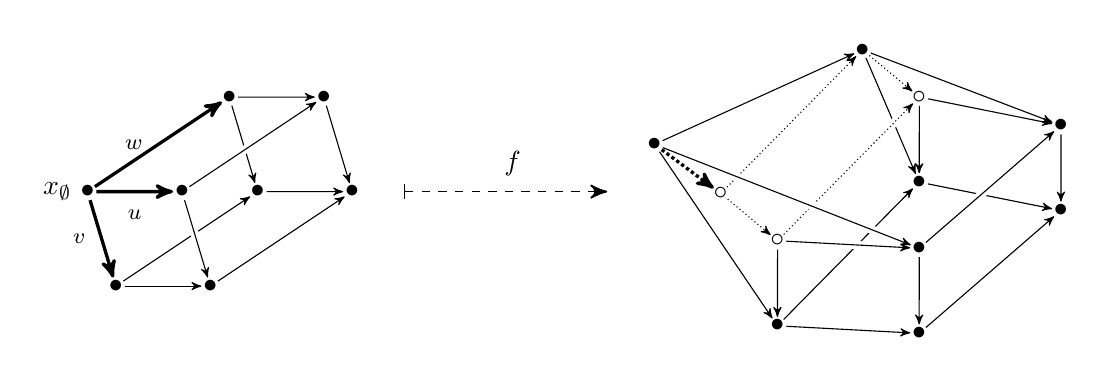
\begin{tikzpicture}[scale=1.2]
\path (0.3,0) node[name=2] {$\bullet $};
\path (1.3,0) node[name=12] {$\bullet $};
\path (0,1) node[name=0d] {$\bullet $};
\path (0d) node[left] {$x_{\emptyset }$};
\path (1,1) node[name=1] {$\bullet $};
\path (1.5,1)+(0.3,0) node[name=23] {$\bullet $};
\path (1.5,1)+(1.3,0) node[name=123] {$\bullet $};
\path (1.5,1)+(0,1) node[name=3] {$\bullet $};
\path (1.5,1)+(1,1) node[name=13] {$\bullet $};

\path[->,very thick] (0d) edge node[below,font=\footnotesize]{$u$} (1);
\path[->,very thick] (0d) edge node[left,font=\footnotesize]{$v$} (2);
\path[->,very thick] (0d) edge node[left,font=\footnotesize]{$w$} (3);

\path[->] (2) edge (12);

\path[->] (3) edge  (23);
\path[->] (3) edge  (13);
\path[->] (13) edge (123);
\path[->] (23) edge (123);


\path[->] (2) edge  (23);
\path[->] (12) edge  (123);

\path[->] (1) edge [-,line width=3pt,draw=white] (12)
			edge (12);
\path[->] (1) edge [-,line width=3pt,draw=white] (13)
			edge (13);

\draw [ |->,dashed, decoration={markings,mark=at position 1 with {\arrow[scale=1.7]{>}}},
    postaction={decorate},
    shorten >=0.4pt
] (3.5,1) -- node[above]{$f$} (5.5,1);

\path (7-1,1.5) node[name=0] {$\bullet $};

\path (7+1.3+.2+.3,1-.5-.1) node[name=1] {$\bullet $};
\path (7+0.3,-0.42) node[name=2] {$\bullet $};
\path (1.5,1)+(7-1+.7,1.8-.3) node[name=3] {$\bullet $};

\path (7+1.3+.2+.3,0-.5) node[name=12] {$\bullet $};
\path (1.5,1)+(7+0.3,.1) node[name=23] {$\bullet $};
\path (1.5,1)+(7+1.3+.5,.7) node[name=13] {$\bullet $};

\path (1.5,1)+(7+1.3+.5,-.2) node[name=123] {$\bullet $};

\path let \p1 = (2), \p2 = (1), \p3=(12) in node[name=pull]  at (\x1+\x2-\x3,\y1+\y2-\y3) {$\circ$};
\path let \p1 = (23), \p2 = (13), \p3=(123) in node[name=pull3]  at (\x1+\x2-\x3,\y1+\y2-\y3) {$\circ$};
\path let \p1 = (3), \p2 = (pull), \p3=(pull3) in node[name=pullpull]  at (\x1+\x2-\x3,\y1+\y2-\y3) {$\circ$};

\path[->] (0) edge (2);
\path[->] (1) edge (12);
\path[->] (2) edge (12);
\path[->] (pull) edge (2);
\path[->,very thick,densely dotted] (0) edge (pullpull);

\path[->] (3) edge (13);
\path[->] (3) edge (23);
\path[->] (13) edge (123);
\path[->] (23) edge (123);
\path[->] (pull3) edge (13);
\path[->] (pull3) edge (23);
\path[->,densely dotted] (3) edge (pull3);
\path[->,densely dotted] (pullpull) edge (pull);
\path[->,densely dotted] (pullpull) edge (3);

\path[->] (0) edge (3);
\path[->] (2) edge (23);
\path[->] (12) edge (123);

\path[->] (pull) edge [-,line width=3pt,draw=white] (pull3);
\path[->,densely dotted] (pull) edge (pull3);
\path[->] (pull) edge [-,line width=3pt,draw=white] (1) edge (1);

\path[->, shorten >=.25cm, shorten <=.25cm] (0) edge [-,line width=3pt,draw=white] (1);
\path[->] (0) edge (1);
\path[->] (1) edge [-,line width=3pt,draw=white] (13) edge (13);


\end{tikzpicture}\\
The dotted vector approximates $\partial_w \partial_v \partial_uf(x_{\emptyset })$.
\end{center}



\end{document}





















































\[{
\def\objectstyle{\scriptstyle}
\def\labelstyle{\scriptstyle}
\xymatrix@R=8mm@C=8mm@!0{
|n+1|^{i}
\ar@{=}[ddd];[]
\ar@{~>}[rrrr];[]
&%r1c1
&%r1c2
&%r1c3
&%r1c4
\|n+1\||n+1|^{i}
\ar@{=}[ddd];[]|!{[dll];[drr]}{\hole}
&%r1c5
&%r1c6
&%r1c7
&%r1c8
|n+1|^{i+1}
\ar@{=}[ddd];[]|!{[dll];[drr]}{\hole}
\ar@{=}[rrrr];[]
\ar[llll];[]
&%r1c9
&%r1c10
&%r1c11
&%r1c12
|n+1|^{i+1}
\ar@{=}[ddd];[]|!{[dll];[drr]}{\hole}
&%r1c13
&&&
|n+1|^{i+1}
\ar@{=}[ddd];[]|!{[dll];[drr]}{\hole}
\ar@{=}[llll];[]
\\%r1c14
&%r2c1
&%r2c2
|n|^i
\ar[ull];[]
\ar[ddd];[]
\ar@{~>}[rrrr];[]
&%r2c3
&%r2c4
&%r2c5
&%r2c6
\|n+1\||n|^i
\ar[ddd];[]
\ar[ull];[]
&%r2c7
&%r2c8
&%r2c9
&%r2c10
|n+1||n|^i
\ar[ddd];[]
\ar[ull];[]
\ar[llll];[]
\ar[rrrr];[]
&%r2c11
&%r2c12
&%r2c13
&%r2c14
|n|^{i+1}
\ar[ull];[]
\ar[ddd];[]
&&&&
|n|^{i+1}
\ar[ddd];[]
\ar@{=}[llll];[]
\ar[ull];[]
\\%r2c15
\\%r3c14
|n+1|^{i}
\ar@{~>}[rrrr];[]|!{[uurr];[drr]}{\hole}
&%r1c1
&%r1c2
&%r1c3
&%r1c4
\|n+1\||n+1|^{i}
&%r1c5
&%r1c6
&%r1c7
&%r1c8
|n+1|^{i+1}
\ar@{=}[rrrr];[]|!{[uurr];[drr]}{\hole}
\ar[llll];[]|!{[uull];[dll]}{\hole}
&%r1c9
&%r1c10
&%r1c11
&%r1c12
|n+1|^{i+1}
&%r1c13
&&&
|n+1|^{i+1}
\ar@{=}[llll];[]|!{[uull];[dll]}{\hole}
\\%r1c14
&%r2c1
&%r2c2
B_n^i
\ar[ull];[]
\ar@{~>}[rrrr];[]
&%r2c3
&%r2c4
&%r2c5
&%r2c6
\|n+1\|B_n^i
\ar[ull];[]
&%r2c7
&%r2c8
&%r2c9
&%r2c10
|n+1|B_n^i
\ar[ull];[]
\ar[llll];[]
\ar@{=}[rrrr];[]
&%r2c11
&%r2c12
&%r2c13
&%r2c14
|n+1|B_n^{i}
\ar[ull];[]
&&&&
B_n^{i+1}
\ar[llll];[]
\ar[ull];[]
\\%r2c15
\\%r6c14
A_{n,i}
\ar[uuu];[]
\ar@{~>}[rrrr];[]|!{[uurr];[drr]}{\hole}
&%r1c1
&%r1c2
&%r1c3
&%r1c4
\|n+1\|A_{n,i}
\ar[uuu];[]|!{[uull];[uurr]}{\hole}
&%r1c5
&%r1c6
&%r1c7
&%r1c8
|n+1|A_{n,i}
\ar[uuu];[]|!{[uull];[uurr]}{\hole}
\ar[rrrr];[]|!{[uurr];[drr]}{\hole}
\ar[llll];[]|!{[uull];[dll]}{\hole}
&%r1c9
&%r1c10
&%r1c11
&%r1c12
A_{n,i+1}
\ar[uuu];[]|!{[uull];[uurr]}{\hole}
\ar@{=}[rrrr];[]|!{[uurr];[drr]}{\hole}
&%r1c13
&&&
A_{n,i+1}
\ar[uuu];[]|!{[uull];[uurr]}{\hole}\\%r1c14
&%r2c1
&%r2c2
A_{n,i}\cap B_n^i
\ar[ull];[]
\ar[uuu];[]
\ar@{~>}[rrrr];[]
&%r2c3
&%r2c4
&%r2c5
&%r2c6
\|n+1\|(A_{n,i}\cap B_n^i)
\ar[uuu];[]
\ar[ull];[]
&%r2c7
&%r2c8
&%r2c9
&%r2c10
|n+1|(A_{n,i}\cap B_n^i)
\ar[uuu];[]
\ar[ull];[]
\ar[llll];[]
\ar[rrrr];[]
&%r2c11
&%r2c12
&%r2c13
&%r2c14
A_{n,i+1}\cap (|n+1|B_n^i)
\ar[ull];[]
\ar[uuu];[]
&&&&
A_{n,i+1}\cap B_n^{i+1}
\ar[llll];[]
\ar[uuu];[]
\ar[llu];[]
\\
&\textup{2.4(i)}&&&
&(\textup{2.4(i)})^{\textup{fat}}&&&
&T_n(\textup{2.4(i)})&&&
&\textup{2.11(i+1)}&&&
&\textup{2.4(i+1)}&
}}\]




%% The orignal
\[{
\def\objectstyle{\scriptstyle}
\def\labelstyle{\scriptstyle}
\xymatrix@R=8mm@C=8mm@!0{
|n+1|^{i}
\ar@{=}[ddd]
\ar@{~>}[rrrr]
&%r1c1
&%r1c2
&%r1c3
&%r1c4
\|n+1\||n+1|^{i}
\ar@{=}[ddd]|!{[dll];[drr]}{\hole}
&%r1c5
&%r1c6
&%r1c7
&%r1c8
|n+1|^{i+1}
\ar@{=}[ddd]|!{[dll];[drr]}{\hole}
\ar@{=}[rrrr]
\ar[llll]
&%r1c9
&%r1c10
&%r1c11
&%r1c12
|n+1|^{i+1}
\ar@{=}[ddd]|!{[dll];[drr]}{\hole}
&%r1c13
&&&
|n+1|^{i+1}
\ar@{=}[ddd]|!{[dll];[drr]}{\hole}
\ar@{=}[llll]
\\%r1c14
&%r2c1
&%r2c2
|n|^i
\ar[ull]
\ar[ddd]
\ar@{~>}[rrrr]
&%r2c3
&%r2c4
&%r2c5
&%r2c6
\|n+1\||n|^i
\ar[ddd]
\ar[ull]
&%r2c7
&%r2c8
&%r2c9
&%r2c10
|n+1||n|^i
\ar[ddd]
\ar[ull]
\ar[llll]
\ar[rrrr]
&%r2c11
&%r2c12
&%r2c13
&%r2c14
|n|^{i+1}
\ar[ull]
\ar[ddd]
&&&&
|n|^{i+1}
\ar[ddd]
\ar@{=}[llll]
\ar[ull]
\\%r2c15
\\%r3c14
|n+1|^{i}
\ar@{~>}[rrrr]|!{[uurr];[drr]}{\hole}
&%r1c1
&%r1c2
&%r1c3
&%r1c4
\|n+1\||n+1|^{i}
&%r1c5
&%r1c6
&%r1c7
&%r1c8
|n+1|^{i+1}
\ar@{=}[rrrr]|!{[uurr];[drr]}{\hole}
\ar[llll]|!{[uull];[dll]}{\hole}
&%r1c9
&%r1c10
&%r1c11
&%r1c12
|n+1|^{i+1}
&%r1c13
&&&
|n+1|^{i+1}
\ar@{=}[llll]|!{[uull];[dll]}{\hole}
\\%r1c14
&%r2c1
&%r2c2
B_n^i
\ar[ull]
\ar@{~>}[rrrr]
&%r2c3
&%r2c4
&%r2c5
&%r2c6
\|n+1\|B_n^i
\ar[ull]
&%r2c7
&%r2c8
&%r2c9
&%r2c10
|n+1|B_n^i
\ar[ull]
\ar[llll]
\ar@{=}[rrrr]
&%r2c11
&%r2c12
&%r2c13
&%r2c14
|n+1|B_n^{i}
\ar[ull]
&&&&
B_n^{i+1}
\ar[llll]
\ar[ull]
\\%r2c15
\\%r6c14
A_{n,i}
\ar[uuu]
\ar@{~>}[rrrr]|!{[uurr];[drr]}{\hole}
&%r1c1
&%r1c2
&%r1c3
&%r1c4
\|n+1\|A_{n,i}
\ar[uuu]|!{[uull];[uurr]}{\hole}
&%r1c5
&%r1c6
&%r1c7
&%r1c8
|n+1|A_{n,i}
\ar[uuu]|!{[uull];[uurr]}{\hole}
\ar[rrrr]|!{[uurr];[drr]}{\hole}
\ar[llll]|!{[uull];[dll]}{\hole}
&%r1c9
&%r1c10
&%r1c11
&%r1c12
A_{n,i+1}
\ar[uuu]|!{[uull];[uurr]}{\hole}
\ar@{=}[rrrr]|!{[uurr];[drr]}{\hole}
&%r1c13
&&&
A_{n,i+1}
\ar[uuu]|!{[uull];[uurr]}{\hole}\\%r1c14
&%r2c1
&%r2c2
A_{n,i}\cap B_n^i
\ar[ull]
\ar[uuu]
\ar@{~>}[rrrr]
&%r2c3
&%r2c4
&%r2c5
&%r2c6
\|n+1\|(A_{n,i}\cap B_n^i)
\ar[uuu]
\ar[ull]
&%r2c7
&%r2c8
&%r2c9
&%r2c10
|n+1|(A_{n,i}\cap B_n^i)
\ar[uuu]
\ar[ull]
\ar[llll]
\ar[rrrr]
&%r2c11
&%r2c12
&%r2c13
&%r2c14
A_{n,i+1}\cap (|n+1|B_n^i)
\ar[ull]
\ar[uuu]
&&&&
A_{n,i+1}\cap B_n^{i+1}
\ar[llll]
\ar[uuu]
\ar[llu]
\\
&\textup{2.4(i)}&&&
&(\textup{2.4(i)})^{\textup{fat}}&&&
&T_n(\textup{2.4(i)})&&&
&\textup{2.11(i+1)}&&&
&\textup{2.4(i+1)}&
}}\]



